\documentclass[12pt,phd,a4paper,oneside]{thesis}

% -------- Packages --------

\usepackage{blindtext}
\usepackage{emptypage}

\usepackage[rgb,dvipsnames]{xcolor}
\usepackage[format=hang,font=small,labelfont=bf,hypcap=false]{caption}
\usepackage{graphicx,tikz,listings,color,float,caption}

\usetikzlibrary{shapes.geometric,arrows}
\restylefloat{figure}
\graphicspath{{figures/}}

\usepackage{amsmath,amssymb,amsfonts,bbold}
\usepackage{booktabs} % pretty tables
\usepackage[version=4]{mhchem}

\usepackage{gensymb}
\usepackage{textcomp}

\usepackage{setspace}
\setstretch{1.5}

\usepackage{multirow}
\usepackage{bibentry} 
\usepackage{etoolbox}

\usepackage[normalem]{ulem}
\usepackage[T1]{fontenc}
\usepackage[utf8]{inputenc}

\let\altmathbb\mathbb
\usepackage[sc]{mathpazo}
\AtBeginDocument{\let\mathbb\altmathbb}

\usepackage{epigraph} %quotes
\usepackage{musixtex}

\setlength\epigraphwidth{.8\textwidth}

\usepackage{notoccite}% PREVENTS CITES IN CAPTIONS FROM MISNUMBERING YOUR REFERENCES 
\usepackage{pdfpages}
\input{FloatSettings} % For things like figures and tables
% defining commands for creating flowcharts
\tikzstyle{startstop} = [rectangle,rounded corners,minimum width=3cm,minimum height=1cm,text centered,draw=black,fill=gray!30]
\tikzstyle{io} = [trapezium, trapezium left angle=70, trapezium right angle=110, minimum width=3cm, minimum height=1cm, text centered, draw=black]
\tikzstyle{process} = [rectangle, minimum width=3cm, minimum height=1cm, text centered, draw=black, fill=gray!30]
\tikzstyle{decision} = [diamond, minimum width=3cm, minimum height=1cm, text centered, draw=black, fill=yellow!30]
\tikzstyle{arrow} = [thick,->,>=stealth]

% defining python syntax highlighting environment
\DeclareFixedFont{\ttb}{T1}{txtt}{bx}{n}{9} % for bold
\DeclareFixedFont{\ttm}{T1}{txtt}{m}{n}{9}  % for normal

% python syntax colors
\definecolor{deepblue}{rgb}{0,0,0.5}
\definecolor{deepred}{rgb}{0.6,0,0}
\definecolor{deepgreen}{rgb}{0,0.5,0}

% Python style for highlighting
\newcommand\pythonstyle{\lstset{
language=Python,
basicstyle=\ttm,
otherkeywords={self},             % Add keywords here
keywordstyle=\ttb\color{deepblue},
emph={MyClass,__init__},          % Custom highlighting
emphstyle=\ttb\color{deepred},    % Custom highlighting style
stringstyle=\color{deepgreen},
frame=tb,                         % Any extra options here
showstringspaces=false            %
}}

% python environment and inline
\lstnewenvironment{python}[1][]{
  \pythonstyle
  \lstset{#1}
}{}
\newcommand\pythoninline[1]{{\pythonstyle\lstinline!#1!}}

% mathematical formatting
\newcommand{\Vector}[1]{\vec{#1}}
\newcommand{\Matrix}[1]{\mathbf{#1}}

\newcommand{\dt}{\mathrm{d}t}

\newcommand{\edit}{\textcolor{blue}}
\newcommand{\stolen}{\textcolor{red}}
\newcommand{\duplicate}{\textcolor{teal}} %duplicate w/ methods in paper(s) -- may need further depth in intro

\newcommand{\rates}{F_{\theta}}
\newcommand{\tangent}{T_{\theta}}
\newcommand{\steadystates}{\partial S_{\theta}}

\newcommand{\Det}{\left| \frac{\partial\rates}{\partial u} \right|}
\newcommand{\measure}{\varphi_{\theta}}

\newcommand{\predictions}{\mathcal{P}}
\newcommand{\targets}{\mathcal{D}}
\newcommand{\loss}{L}
\newcommand{\error}{E}
\newcommand{\Reals}{\mathbb{R}}
\newcommand{\steady}{u^*}
\newcommand{\cycle}{\omega}
\newcommand{\jacobian}{\frac{\partial\rates}{\partial u}}
\newcommand{\eigenvector}{\hat{v}_\lambda}
\newcommand{\e}{\mathbb{e}}

\makeatletter
\AtBeginDocument{
    \hypersetup{
        pdfsubject={Biophysics},
        pdfkeywords={inference,bifurcations},
        pdfauthor={Grisha Szep},
        pdftitle={Inferring bifurcations between phenotypes},
    }
}
\makeatother

\bibliographystyle{unsrt}  % For bibliographies
\setcounter{secnumdepth}{3}
\setcounter{tocdepth}{3}
\setboolean{@twoside}{false}

\begin{document}
\raggedbottom % stops huge gaps between paragraphs

\title{Inferring bifurcations\\between phenotypes}
\author{Grisha Szep}

\department{Randall Division of Cell \& Molecular Biophysics}
\sponsor{Microsoft Research Cambridge}

\date{October 29, 2021}
\maketitle
% \makedeclaration

\begin{abstract} % 300 word limit

    The gene-expression history of an organism and its environment determine the organism's phenotype. The phenotype is an inherently qualitative state, deduced by relative biochemical concentration measurements collected by methods such as flow cytometry or fluorescence microscopy. The biochemical threshold concentrations that distinguish different phenotypes can be modelled by applying bifurcation analysis to differential equation models and the search for these boundaries in experimental data can be done using dimensionality reduction and clustering techniques. This establishes a relationship between bifurcations, phenotypes and machine learning techniques that are the subject of this thesis.

    % The first chapter presents an interactive tool for exploring phenotypes in flow cytometry data. In particular we explore a multi-tissue, high-dimensional, immune cell dataset. The tool bridges machine learning methods and the popular FlowJo, used to annotate cells with gating strategies. An assortment of dimensionality reduction techniques are applied to create two dimensional embeddings and confusion matrices are used to quantify annotation agreement between immunologists. By leveraging the geospatial mapping library OpenLayers to render, annotate and analyze cells, immunologists can now efficiently navigate the phenotype space of Human Cell Atlas datasets.
    
    % The next chapter focuses on a model-driven approach for exploring and designing phenotypes, where we demonstrate how model-guided design of synthetic E. Coli can elucidate pattern formation mechanisms in multicellular development. We infer the parameters of a biochemically motivated system of differential equations against time course fluorescence data acquired from plate reader experiments. Our design goals however were not in the temporal domain, rather we wanted to control the shape and size of a cusp bifurcation in the space of experimentally controlled input concentrations.
    
    % To address these limitations, I define a differentiable semi-supervised cost function that uses bifurcation locations as targets. Bifurcations are encouraged by an unsupervised term that extremises the curvature of the determinant of the Jacobian. By exploring the cost landscape for minimal models that span the space of saddle-nodes and pitchforks, I show that the parameter space basins define regions of qualitatively equivalent differential equations. The differentiability of the cost function enables efficient optimisation using libraries such as Flux.jl that leverage automatic differentiation. The impact of this work would enable experimentalists to efficiently navigate design spaces of differential equation models.
    
\end{abstract}
\newpage
\clearpage
\begin{center}
    \thispagestyle{empty}
    \vspace*{\fill}
    \epigraph{
        Blank pages are the worst.\\
        They impose a glaring responsibility onto someone to fill it with meaningful content.\\
        Much like other starting points:
        a new job, a marble stone, empty land, all future that tower over you, forcing the person facing it to ask:\\
        "do I really want to do this?"\\
        Blank pages are the worst.\\
        They reflect a glaring light upon you, reflecting the messages that would otherwise happinly bounce around in the ether, along with memories, desires, unfinished projects, and other concofonous bullshit in your head.\\
        A whole page!\\
        Rejoice at the etchings of achievement. You've started now so don't give up, or stop, you'll look stupid. Now make sure you go back and edit the previous page so that other will not know how stupid you are.\\
        Edit it, edit it,\\
        edit it into oblivion untill you can't recognise whether you are editing the page or yourself.}{}
    \vspace*{\fill}
\end{center}
\clearpage

\begin{acknowledgements}
    The past four years of my life have been full of excitement, creativity and exploration, none of which would have been possible without the support of Attila and Neil. Their mentorship and guidance has been a shining example of leadership and whose qualities I will take with me into future roles. I would like to thank my colleagues and friends at Microsoft Research, whose diverse projects in biotechnology captured my imagination.

    I would like to acknowledge Valerie Coppard, who was an absolute pleasure to work with and introduced me to Joanne Jones' lab at Cambridge University, catalysing the \emph{FlowAtlas.jl} project. Her enthusiasm...

    I would like to thank Matilda Peruzzo and Silvia Cabaliero During the pandemic. I would like to thank Mohammed Ali

    I am thankful to my friends at Burnt Umber who run a cozy and welcoming cafe in Hackney Wick, where I wrote a large chunk of my thesis, felt supported and cared for during difficult times. Disree Shaw my therapist. Fraser...

    I would like to thank family and dad
\end{acknowledgements}

%%%%%%%%%%%%%%%%%%%%%%%%%%%%%%%%%%%%%%%%
%%%%%%%%%%%%%%%%%%%%%%%%%%%%%%%%%%%%%%%%
%%%%%%%%%%%%%%%%%%%%%%%%%%%%%%%%%%%%%%%%
%%%%%%%%%%%%%%%%%%%%%%%%%%%%%%%%%%%%%%%%
%%%%%%%%%%%%%%%%%%%%%%%%%%%%%%%%%%%%%%%%

\setcounter{tocdepth}{2} 
% Setting this higher means you get contents entries for
%  more minor section headers.

\tableofcontents
\listoffigures
\chapter{Introduction \& Motivation}
\label{chapter:introduction}
\begin{music}
    \parindent10mm \instrumentnumber{1} \setstaffs1{1} 
    \generalmeter{\meterfrac34} \generalsignature{3}
    \startextract
            \Notes \Dqbu dk \zhl{i*} \en
        \bar
            \Notes \Dqbu hi \zhu{h*} \en
    \zendextract
\end{music}
\epigraph{\textit{one thing that won't change with time is the memories of younger years}}{Minuet of Forest --- Ocarina of Time}

We are living in the wake of milestones in biotechnology and computational biology that suggest reverse-engineering cell biology is within our grasp. The coronavirus pandemic accelerated investment in biotechnology \cite{DeFrancesco2021Financing2020}. The fields of synthetic and systems biology are beginning to resemble engineering disciplines; genetic engineering is becoming more precise, high-throughput single-cell experiments are performed by robots and measurements across all levels of the central dogma are possible: genomics, transcriptomics, proteomics and metabolomics \cite{Perkel2021Single-cellAge}. Advances in micro-fabrication \cite{Shafiee2017TissueMedicine} and in-vitro reconstitutive methods \cite{Gopfrich2018MasteringCells} have allowed biologists isolate pathways and mechanisms to a level of mathematical and computational tractability \cite{Sharpe2017ComputerTomorrow.}.

The complexity barrier in biology poses a significant challenge. Systems and synthetic biology have historically made progress through a process of brute force trial and error. This usually involves the interaction of many custom-made parts that are iteratively optimised by human intervention. A trend first observed in the 1980s known as \textit{Eroom's law} revealed that discoveries in biotechnology are becoming slower and more expensive over time, despite improvements in technology \cite{Scannell2012DiagnosingEfficiency}. This problem is exemplified by the declining success rate of clinical trials in the drug discovery process \cite{Wong2019EstimationParameters} and compounded by the ongoing reproducibility crisis \cite{Ioannidis2005WhyFalse.,Mullard2021HalfEffort}. It appears that much of the low-hanging fruit has been picked \cite{Earm2014IntegrativeDevelopment} with methodologies whose standards for transparency, reproducibility and accessibility leave us with much to be desired. Despite the widespread lack of mechanistic understanding in human cell biology, sophisticated engineering goals such as targeted modification of the immune system are now possible. In 2018, a chimeric antigen receptor T-cell therapy --- \emph{tisagenlecleucel} \cite{Halford2021TisagenlecleucelConsiderations} --- for the treatment of adolescent and young adult acute lymphoblastic leukaemia became the most expensive cancer therapy ever, at \$475,000. In settings where biomanufacturing relies on specific known mechanisms, but otherwise involve a greater number of unknown mechanisms, a vast amount of omics data is collected along key protocol stages in a attempts to understand and optimise production.

After a decade of engineering advances in data science and machine learning, epitomised by deep learning methods, theoretical foundations on high-dimensional learning tasks are beginning to condense \cite{Bronstein2021GeometricGauges}. Many tasks such as computer vision, playing Go, or protein folding are in fact feasible with appropriate computational scale. Remarkably, the essence of deep learning is built from two simple algorithmic principles: the notion of lower-dimensional \emph{representation}, whereby group equivariant and invariant transformations are composed to capture the appropriate notion of regularity for each task \cite{Bronstein2021GeometricGauges}, and second, learning by local gradient-descent type methods enabled by \emph{differentiable programming} \cite{Innes2019AComputing}.

The emerging picture suggests that bringing together the advances in software and wetware in iterative hypothesis generation and discovery pipelines are key to overcoming the complexity barrier in biology \cite{Sharpe2017ComputerTomorrow.,Ringel2020BreakingLaw,AlQuraishi2021DifferentiableMechanisms}. The term \textit{in silico} has become popularised amongst biologists, which conceptualises a computational model, alongside \emph{in vitro} and \emph{in vivo}, as a method for investigating an organism \emph{in situ}. Researchers are going as far as conceptualising the \emph{digital twin} for personalised medicine \cite{Bjornsson2019DigitalMedicine}. Bringing together deep learning and biomedical research has the potential of importing the notions of \emph{representation} and \emph{differentiability} into experimental protocols \cite{AlQuraishi2021DifferentiableMechanisms} and thereby reaping their benefits. Differentiability within experimental pipelines has the same advantage over brute force trial and error as it does over sampling-based algorithms and thereby decrease the time and cost for biological research. While not all equipment, data and resources used to perform a study can be shared, representations of a study in the form of computational models can increase transparency and reproducibility. Efforts towards open standards have gained traction over the past decade \cite{Malik-Sheriff2020BioModels15Science} with model sharing standards such as Systems Biology Markup Language \cite{Hucka2018TheCore} and data repositories like Human Cell Atlas
\cite{Regev2017TheAtlas} and Flow Repository \cite{Spidlen2012PreparingFlowRepository.org}. The open standards and ethical thresholds of deep learning are also increasing, with the formation of OpenAI \cite{Brockman2016OpenAIGym} and sharing standards such as ONNX \cite{Bai2019ONNX:Exchange}.

\section{Representation of Single Cells}

In this thesis, the focus is on differential equation representations of single cells. In this section we give a brief motivation behind why differenital equations are convenient, what other representations exist and how results may translate between differenital equations and other representations. When studying a particular biological phenomenon, the appropriate spatio-temporal scale must be chosen that simplifies the mechanism under study while preserving the relationships between experimentally accessible parameters and the resultant behaviours. We do not expect a single unifying tractable model of biological mechanisms under study. In practice there exist multiple equally valid models with variously degrees of complexity.
\begin{Figure}
    \includegraphics[width=0.9\linewidth]{figures/top-down-bottom-up}
    \caption{Biological models at different spatial scales and complexities, a large class of which can be cast into differential equation form indicated in bold blue}
    \label{fig:tdbu}
\end{Figure}
Differential equations are convenient because they are differentiable, continuous state and continuous time models and hence are already compatible with the two algorithmic principles of deep learning \cite{Bronstein2021GeometricGauges}. In the context of dynamical systems theory it is relatively simple to derive analogous results for descrete state or descrete time models: cellular automata \cite{Martin2017DifferentiableAutomata}, markov chains \cite{Darling2008DifferentialChains}, stocastic processes and descrete maps just to name a few. A large class of biological models at different spatial scales can be cast into differential equation form (Figure \ref{fig:tdbu}), although this may not always be necessary. With the help of automatic differentiation, programs with arbitrary control flow become piecewise differentiable \cite{Gune2018AutomaticSurvey}. One of the main limitations to consider is the number of branches in the program due to conditional statements and whether there are non-zero derivatives either side of the conditional statement that provide meaningful information. Rule-based models such as agent-based models are examples of programs with many conditional branches often with no meaningful derivatives on either side of the condition. In such scenarios we must fall back to finite difference approaches, requiring a finite number of evaluations of the model. This can be done in a cost-effective way, only evaluating gradients that will likely benefit the optimisation.

Differential equations models span a large range of spatial and temporal scales. It is important to choose a time-scale and space-scale that is relevant to the problem. If one is interested in tissue dynamics, attempting to model DNA conformations within each cell will render the problem intractable. As George Booth aptly put \textit{``most models are wrong but some are useful"} so the role of theoretical descriptions in these settings is not necessarily to describe the way reality \textit{is} but serve as tools to bridge the non-intuitive gap between bottom-up and top-down approaches \cite{Gopfrich2018MasteringCells,Powell2018HowScratch,Pezzulo2016Top-downLevel}.

\subsection{Model Selection \& Reduction}
With such a hetergenous selection of models that are valid at different spatial and temporal scales it becomes increasingly important to develop tools to navigate the space of models. This problem is known in machine learning as model selection \cite{Ding2018ModelOverview} and establishing relationships between models of varying complexity is know as model reduction \cite{Besselink2013AControl}. We will see in the following section that exploring the space of models inherently involves some form of iterative hypothesis generation workflow.

In the context of parameter inference \cite{Brunton2016SparseSINDYc,GorbachScalableSystems}, sloppiness and sensitivity analysis have been extensively used in the search for reduced models \cite{Daniels2008,Chis2016OnIdentifiability,Gutenkunst2007UniversallyModels,Gabor2017ParameterBiosystems,Villaverde2016StructuralModels}. Linear mappings between models that preserve stoichiometry and reactant structure were investigated \cite{Cardelli2014MorphismsFunction,Cardelli2017MaximalSystems} and computational tools based on partition-refinement were released \cite{Cardelli2017ERODE:Equations}. Structural similarity between reaction networks can be revealed by such mappings, elucidating the functional aspects of complex networks in terms of simpler networks. Nonlinear mappings between models that preserve high-level features without resorting to structural assumptions about the models were still lacking lacking and formed part of the motivation for developing the methods in Chapter \ref{chapter:inference}.

We will see how a suitably defined cost function that focuses on high-level features of a model enables navigation and organisation of models across various levels of complexity. Indeed the focus on higher-level features of differential equation models, such as geometry rather than kinetics, has already been gaining traction in 
pattern formation theory \cite{Halatek2018}.

\section{Differentiability in Experimental Protocols}

While there is a clear mathematical definition of what a \emph{differentiable program} \cite{Innes2019AComputing} is, what does it mean for experimental protocols in biology to be differentiable? In the effort to move past brute force trial and error methods, a standard for the \emph{design--build--test--learn} cycle has emerged in synthetic biology (Figure \ref{fig:dbtl}). This workflow has now been established as a paradigm \cite{Carbonell2018AnChemicals,Opgenorth2019LessonsLearning} with some aspects that have been automated by liquid handling robots, bioreactor environments and image processing pipelines. However, humans in the loop and custom moving parts still persist. Defining the boundary between parts that can be automated, and parts that need regular intervention by domain experts is a challenge \cite{Abate2018ExperimentalSemantics}.
\begin{Figure}
    \includegraphics[width=0.6\linewidth]{figures/dbtl}
    \caption{\emph{design--build--test--learn} cycle from synthetic biology. This cycle is differentiable if a domain expert can track changes in any observation pair \emph{X,Y} along the pipeline}
    \label{fig:dbtl}
\end{Figure}
In principle such a pipeline is differentiable if a domain expert can efficiently get an answer questions like: \emph{What happens to Y when I change X?} or \emph{Which X do need to change in order to change Y?} for as many observable pairs \emph{X,Y} as possible. Furthermore, suitable experiments are identified to the capture the relevant data.

The \emph{design--build--test--learn} paradigm was used during the interdisciplinary collaboration described in Chapter \ref{chapter:double-exclusive}. In this thesis we focus on the \emph{design--learn} part of this workflow. One of the main learnings, as we shall see, from applying this paradigm is that, in order for the lab to converge onto their cell design goals efficiently, the workflow must be bidirectional, rather than a cycle. This way each part of the workflow can operate with its neighbours indepentently, without being blocked by other parts of the workflow.

\subsection{Design--Learn Workflow}
\label{section:design-learn}
Let us focus on the \emph{design--learn} part of the workflow in the context of model inference. Partial knowledge of mechanisms in biology has given rise to a class of models that have been coided as \emph{grey box models} \cite{Meeds2019EfficientSystems}. In this setting, domain expertise dictates which aspects of the model are highly structured with specific hypotheses and which are composed with generic transformations that obey a chosen set of group symmetries.
\begin{Figure}
    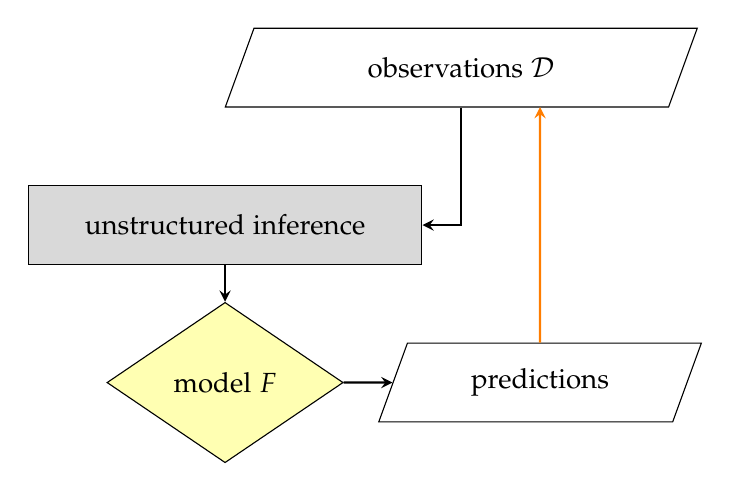
\begin{tikzpicture}[node distance=2cm]

        \node (nonparametric) [process, minimum width=5cm] {unstructured inference};
        \node (data) [io, right of=nonparametric, xshift=1cm, yshift=2cm] {observations $\mathcal{D}$};

        \node (field) [decision, below of=nonparametric] {model $F$};
        \node (pred) [io, right of=field,  xshift=2cm] {predictions};

        \draw [arrow] (data) |- (nonparametric);
        \draw [arrow] (nonparametric) -- (field);
        
        \draw [arrow] (field) -- (pred);
        \draw [arrow,color=BurntOrange] (pred) -- +(0,3.5);

    \end{tikzpicture}
    \caption{\emph{Design--learn} workflow without mechanistic knowledge. Predictions generated from the model $F$ are only accurate in the vicinity of data $\targets$}
    \label{fig:experimental-design}
\end{Figure}
Suppose our collaborators have provided us with time-course gene expression data $\mathcal{D}$, which could be taken via time-lapse microscopy of cells growing on microfluidic plates, optical density measurements from microtiter plate assays or temporal snapshots of flow cytometry measruements. If nothing is known about a mechanism under study, we can infer an unstructured model from a set of observations, and even generate predictions without needing to know anything about the mechanism (Figure \ref{fig:experimental-design}). Unstructured models do not generate accurate predictions outside the input data distribution; they are good interpolars, but terrible extrapolators.

Models $\rates$ constructed with feasible biophysical assumptions have the potential to extrapolate predictions and give concrete biophysical meanings to each parameter $\theta$. This way the experimentalist knows exactly which modification to the system they must make in order to achieve a desired behaviour. More often than not it is also unclear whether the model and its assumptions are reasonable, which brings us to model selection and reduction (Figure \ref{fig:non-parametric}). 
\begin{Figure}
    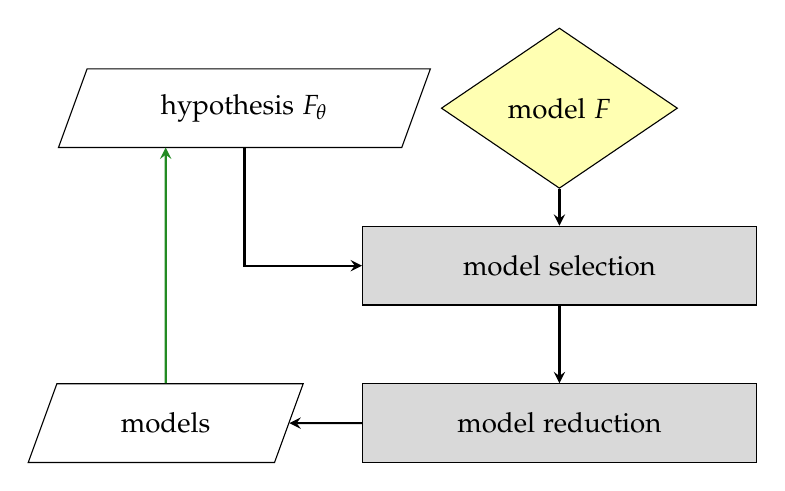
\begin{tikzpicture}[node distance=2cm]

        \node (field) [decision] {model $F$};
        \node (hypothesis) [io, left of=field,  xshift=-2cm] {hypothesis $\rates$};
        \node (parametric) [process, below of=field, minimum width=5cm] {model selection};
        
        \node (decomp) [process, below of=parametric, minimum width=5cm] {model reduction};
        \node (models) [io, left of=decomp, xshift=-3cm] {models};

        \draw [arrow] (field) -- (parametric);
        \draw [arrow] (hypothesis) |- (parametric);
        \draw [arrow] (parametric) -- (decomp);
        
        \draw [arrow] (decomp) -- (models);
        \draw [arrow,color=ForestGreen] (models) -- +(0,3.5);

    \end{tikzpicture}
    \caption{Overview of model selection, reduction and refinement loop}
    \label{fig:non-parametric}
\end{Figure}
Alternatively one may construct $\rates$ to cover a whole class of models rather than a single model. The expectation is that most of the parameters would be zero but some would be informative \cite{Brunton2016SparseSINDYc}. From the inferred parameters $\theta$ one may construct alternative hypotheses and narrow down the set of plausible models. By iterating this procedure one would identify the minimal model within the model class that explains the data.

In this thesis we focus on the benefits of representation and differentiability in the context of the genetic engineering of cell phenotypes in synthetic biology. In Chapter \ref{chapter:background} we introduce the reader a relevant background in differential equations and machine learning with applications in cell biology to set the stage for the publications in Chapters \ref{chapter:double-exclusive}--\ref{chapter:exploring}. We will see how a differential equation representation of a cell or population of cells requires an exploration of the relationship between bifurcation theory and the concept of a phenotype. Chapter \ref{chapter:double-exclusive} exhibits the results of an interdisciplicary collaboration between in synthetic biology, during which an iterative \emph{design--learn} workflow was followed in an attempt to overcome the biological complexity barrier. During this collaboration, a disconnect between design goals and parameter inference methods was identified which lead to the novel bifurcation inference method published in Chapter \ref{chapter:inference}. Chapter \ref{chapter:exploring} is an adaptation of a publication, in preparation at the time of writing this document, that explores the importance of interactive exploration of high-dimensional flow cytometry data for immunophenotyping. Finally, Chapter \ref{chapter:conclusions} concludes with retrospectives on the previous chapters, which includes a revised view of a \emph{design--learn} workflow for synthetic biology, that in principle is completely differentiable. Furthermore, we propose how one would use concepts from Chapters \ref{chapter:inference}--\ref{chapter:exploring} to interactivity explore the space of hypotheses that represent the same cell phenotype. Our conclusions would be most impactful in cell line development where flow cytometry and other omic-type measurements are taken at different protocol stages of a biomanufacturing process.

% On the other hand one may want to specify a behaviour
% $\mathcal{H}$ which may have not yet been observed. This would be specified with
% top-down constraints, i.e. there exist oscillations of a fixed frequency or
% a region of bistability.

% The experimentalists may want to know whether the data collected could
% result in a model of predictive power without mechanistic knowledge
% of the underlying biochemistry. Moreover it would be desirable gain insights
% in parameter regimes in the vicinity of observations, without having to
% wait for the theorists to produce a refined model. Such real-time insights
% would guide data collection protocols, optimising the amount of information
% gained while keeping the number of experiments performed to a minimum. Often
% data is noisy and at worst case contradictory; these issues must also be exposed.

% \noindent
% Figure \ref{fig:experimental-design} outlines the workflow for optimal experimental design.
% The term \textit{non-parametric} defines the procedures that have prioritised  
% functional generality and flexibility over mechanistic insights gained from the values
% of the parameters and shapes of the mathematical forms. Neural networks and Gaussian process
% regressors are examples of non-parametric estimation procedures, which produce an estimate
% of the field $\Vector{f}$ that predicts gene expression rates at given expression levels.
% Based on these predictions, the experimentalist may proceed to collect data in the most
% informative parameter regions, which would in turn more accurately estimate $\Vector{f}$.


% Suppose now that refined mechanistic models of the form $\Vector{h}(\Vector{\theta})$
% have been obtained using the model refinement loop. These could be a library of known
% parts that have been individually characterised, but never combined to form a larger
% system. The experimentalists would like to create a system with a specified behaviour
% $\mathcal{H}$ and would like to know which parts to combine and which modifications
% to make. The model refinement loop can be used with the design as an input.

% \begin{Figure}
%     \begin{tikzpicture}[node distance=2cm]

%         \node (nonparametric) [process, minimum width=5cm] {non-parametric inference};
%         \node (design) [io, left of=nonparametric, xshift=-1cm, yshift=2cm] {design $\mathcal{H}$};

%         \node (field) [decision, below of=nonparametric] {field $\Vector{f}$};
%         \node (hypothesis) [io, left of=field,  xshift=-2cm] {models $\Vector{h}(\Vector{\theta})$};
%         \node (parametric) [process, below of=field, minimum width=5cm] {geometric inference};
        
%         \node (params) [io, below of=parametric] {parameter distribution $\rho(\Vector{\theta})$};

%         \draw [arrow] (design) |- (nonparametric);
%         \draw [arrow] (nonparametric) -- (field);
        
%         \draw [arrow] (field) -- (parametric);
%         \draw [arrow] (hypothesis) |- (parametric);
%         \draw [arrow] (parametric) -- (params);

%     \end{tikzpicture}
%     \caption{Overview of system design pipeline}
%     \label{fig:design}
% \end{Figure}
\chapter{Theoretical Background}
\label{chapter:background}
\begin{music}
    \parindent10mm \instrumentnumber{1} \setstaffs1{1} 
    \generalmeter{\meterfrac34} \generalsignature{-1}
    \startextract
		\notes  \en
    \zendextract
\end{music}
\epigraph{\textit{the passion of friendship will soon blossom into a righteous power}}{Bolero of Fire --- Ocarina of Time}

% Convolutional neural networks trained on large databases \cite{mnist2012,imagenet2009} have shaped machine learning research over the past couple of decades. Today they serve as canonical learning material in courses and are often used as initial \textit{vanilla} approaches for data exploration and classification tasks and before creating more bespoke machine learning pipelines. The widespread success of much models created an expectation in the research community that with sufficient data and computational power provided by one of the reigning consumer internet businesses, a data-driven black-box model can be created for any application ranging from quantum mechanics to economics. Convolutional architectures together with language models eventually inspired recurrent architectures and attention models where are the key ingredients in the creation of \textit{Alpha Fold} \cite{Jumper2021HighlyAlphaFold} that takes a substantial step towards solving the protein-folding problem. Biotechnology researchers are eager to apply these methods but face the following obstacles

% \begin{itemize}
%     \item \textbf{Insufficient data} due to strategic experimental designs 
%     \item \textbf{Low extrapolation accuracy} for black box-models
% \end{itemize}

This Chapter lays out a background bifurcation theory and machine learning methods relevant to cell biology and flow cytometry. We establish the connection between the concept of phenotypes and bifurcations in Section \ref{section:phenotypes-with-bifurcations} and lay out assumptions and definitions that are used throughout other chapters. Section \ref{section:applications-cell-biology} follows up with concrete applications of differential equations in cell biology and will prepare the reader for the incorporated synthetic biology publication in Chapter \ref{chapter:double-exclusive}.

The problem of inferring phenotypes from data is defined in Section \ref{section:phenotype-inference} with a survey relevant machine learning methods. This section discusses the pre-processing techniques to extract bifurcations from raw data, as has been done in Chapter \ref{chapter:double-exclusive}, and used as a starting point in the incorporated machine learning publication in Chapter \ref{chapter:inference}. Section \ref{section:applications-flow-cytometry} gives the reader a background in flow cytometry and how the machine learning methods discussed in previous sections are used by immunologists to identify immune cell phenotypes. This section lays the foundations for the interactive exploration tool presented in Chapter \ref{chapter:exploring}.

\section{Describing Phenotypes with Bifurcations}
\label{section:phenotypes-with-bifurcations}

%Bringing in the definition here is too early. Too abrupt.
%Historical context of how the word emerged and how it is used in biological contexts
A phenotype is a qualitative state or behaviour of an organism that can be described by several quantitative features. Before considering the additional complexity that comes with biology, let us first consider a simple everyday metaphor: light bulbs. Light bulbs come in various combinations of quantitative features $\theta$ which could be its shape, colour, materials and circuit design. The purpose of a light bulb is to fulfil a single function: increase in brightness as a function of voltage $p$, pushing the qualitative state of the bulb from \emph{off} to \emph{on}. Changes to bulb shape affect neither its function nor its states. Changes in color affect the quality of the \emph{on} state but not the \emph{off} state. Changes to circuit design and materials may change or even break the bulb's function. Fluorescent bulbs, for example, only have two possible brightness states in response to changes in voltage $p$, while incandescent bulbs have a continuous brightness response.
\\
\begin{Figure}
\includegraphics[scale=0.7]{bulb}
\caption{a) The bifurcations (shown in gold) at critical voltage $p^\star$ above argon concentration $\theta^\star$ give rise to sudden jumps in brightness (right-hand panels). $\theta^\star$ separates two bulb phenotypes and $p^\star$ separates the \emph{on} and \emph{off} states.}
\label{fig:bulb}
\end{Figure}

The fluorescent and incandescent bulbs can be considered as two different phenotypes distinguished by the quality of their response to voltage changes. Different colour bulbs can also be considered phenotypes, distinguished by the quality of their \emph{on} state, rather than their response to voltage. Bifurcation theory allows us to describe the transitions between qualitative states and can be leveraged to distinguish and organise phenotypes. In this context a bifurcation becomes a punctuation that either \emph{distinguishes between phenotypes} or \emph{distinguishes between behaviours within a phenotype}.

Suppose we inserted a component into our light bulb that changed parameter $\theta$ in such a way so that we can change between the discrete response of the fluorescent bulb and the continuous response of the incandescent bulb. Perhaps $\theta$ could be the concentration of argon gas; the bulb would have to be wired to behave like an incandescent bulb at low concentrations. We could collect brightness $u$ as a function of voltage $p$ and gas concentration $\theta$ produce something similar to that shown in Figure \ref{fig:bulb}. The bifurcations at critical voltage $p^\star$ above argon concentration $\theta^\star$ give rise to sudden jumps in brightness. The bifurcations separate the \emph{on} and \emph{off} states of the bulb and are only present in the fluorescent phenotype. The two phenotypes lie either side of  the onset of bifurcations at concentration $\theta^\star$. We can see from Figure \ref{fig:bulb} how knowing the locations of bifurcations allows us to organise qualitative behaviours and hence phenotypes of the bulb.

In the biological context, we can consider changes in $\theta$ as changes in the organism genotype that may or may not lead to a new phenotype. The idea of describing phenotypes in this way has been done before by Waddington \cite{}. His epigenetic landscape is a metaphor for how changes gene regulation, in our case represented by changes in $\theta$, determines the fate of cells. He imagines the cell as a marble, rolling down a series of forking valleys representing a differentiation cascade, eventually settling in its final phenotype. Let us adopt this metaphor for organism behaviours in response to a controlled condition (Figure \ref{fig:waddington}). Changing the control condition places the marble at different points in the valley and each fork in the valley corresponds to different available behaviours to the organism. Changing the parameters $\theta$ changes the topology of the valleys potentially giving rise to new behaviours and therefore new phenotypes. Due to the robustness \cite{} and fragility \cite{} of organisms we expect most changes in $\theta$ to either kill the organism or do nothing at all. The emerging picture suggests that the route between phenotypes is a carefully created sequence of changes in $\theta$.

\begin{Figure}
\includegraphics[scale=0.6]{waddington}
\caption{Waddington landscapes representing the set of available behaviours for two phenotypes in response to a controlled condition $p$. Phenotypes are related by changes in landscape topology via changes in $\theta$}
\label{fig:waddington}
\end{Figure}

In order to enumerate the phenotype distribution in the the high-dimensional parameter space $\theta$ for a given organism we must construct a model. By parametrising such a model $\rates(u,p)$ by $\theta$, we can relate the states of the organism $u$ to experimentally controlled conditions $p$. Ideally a subset of $u$ can be observed experimentally so that we may observe bifurcations in the data, as demonstrated in the right-hand panel of Figure \ref{fig:bulb}. In the following section we shall go through a class of models that can leverage bifurcation theory.  

% The problem is that the space of decisions that change $\theta$ is intractably large. Furthermore there is no guarantee that any two phenotypes would be connected via experimentally accessible changes in $\theta$. We will see in the incorporated publication in Chapter \ref{chapter:double-exclusive} how differential equation modelling and machine learning can be used to guide experiments and the genetic engineering of \emph{E. coli} towards a phenotype referred to as the \emph{double exclusive reporter}. 

% In the collaboration, bifurcation theory \cite{} was used to detect the onset of the desired phenotypic behaviour in a set of differential equations that model the engineered genetic circuits in \emph{E. coli}. We will see in the following sections how bifurcation theory is perfectly suited for modelling transitions between phenotypes, and hence popularised in fields such as synthetic biology and ecology. Through the use of machine learning and bifurcation theory in the same collaboration, we identified a gap: \emph{there existed no differentiable machine learning method that leveraged bifurcation theory directly}. The incorporated publication in Chapter \ref{chapter:inference} fills this gap, enabling an efficient exploration of phenotypes in the high-dimensional space of $\theta$.

% The antimicrobial resistance originates from selective pressures in the environment which change biochemical pathways which we can encode in parameters $\theta$. Neurons also have pathways that regulate aspects such as thickness of myelin sheaths on axons, that in turn dictate how sensitive, if at all, they are to firing. In the case of the \emph{Zebrafish} the parameters $\theta$ encode whether a particular mutation in the genome is present or not. 

% Synthetic biologists like to import such engineering metaphors when designing genetic sequences that would produce a desired behaviour. Genetic components are designed to be modular and mass produced like electrical components. with various behaviours are mass produced.

% This could be, for example, a phenotype of antimicrobial resistant bacteria \cite{Baym2016SpatiotemporalLandscapes}. We can break down this observation as follows: a cell can be in the qualitative state of \emph{resistant} or \emph{not resistant} at a certain concentration $p$ of antibiotic. Another example could be that of action potentials in neurons \cite{}. A neuron can either be \emph{firing} or \emph{not firing} in response to a given electro-chemical potential $p$. Whole organism phenotypes, such as pigment patterns \emph{Zebrafish} \cite{}, can also be described this way. In this case the phenotype emerges as the organism develops and therefore we look for emergence of \emph{patterns} or \emph{no patterns} over time $p=t$.

% In practice we can only observe a subset of the states, for example by incorporating fluorescent proteins downstream of the coding sequences of the proteins that participate in the antimicrobial resistance. Incorporating any fluorescent proteins into the host genome contributes to cell burdon and at worst can disrupt the mechanism under study. Therefore incorporation sites much be chosen sparsely such that the qualitative behaviour is still observable in the data.

\clearpage
\subsection{Differential Equation Models}

For the purposes of this thesis we will assume that the behaviour of the organism under study can be cast in terms of differential equations in a $N$ states $u$, $M$ parameters $\theta$ and $P$ control conditions $p$. For now we shall state the general class of models and follow up with concrete biological examples as we explore different types of bifurcations. Throughout the thesis we will consider models of the form

\begin{equation}
	\frac{du}{dt} = \rates(u,p)
	\where
	\begin{cases}
		\quad F: \Reals^{N+P}\rightarrow\Reals^N \\
		\quad \theta\in\Reals^M, u\in\Reals^N, p\in\Reals^P
	\end{cases}
	\label{eq:differential-equations}
\end{equation}

\noindent The total derivative $\frac{du}{dt}$ gives us the rate of change of the states with respect to time $t$ and all variables have been vectorised with the appropriate dimension. In principle the right-hand-side $\rates$ can be arbitrarily complicated, containing spatial derivatives or even machine learning models such as neural networks. We shall see later when such models become relevant in biomedical modelling.

\subsubsection{Trajectories \& Field Geometry}

In principle once equations \eqref{eq:differential-equations} have been written down they can be integrated to obtain trajectories $u(t)$ for various initial conditions $u(t')$. We can write the solution down formally as
\begin{equation}
	u(t) = u(t') + \int_{t'}^{t} \rates(u(s),p)\,\mathrm{d}s
	\label{eq:trajectory}
\end{equation}
Here the integral reveals that in order to determine where the state is at time $t$ we need to sum all the contributions of the function $\rates$ from the initial time $t'$ all the way up to final time $t$. The function $\rates$ depends on the state $u$ and must be updated with the integration variable $s$. This calculation can be interpreted, as shown in Figure \ref{fig:fields}, as choosing an initial point $u'=u(t')$ in a vector field $\rates$ and following the field lines until time $t$ at which the final point $u=u(t)$ has been reached.

\begin{Figure}
\includegraphics[scale=0.9]{fields}
\caption{Illustration of a trajectory between $u=u(t)$ and $u'=u(t')$ over finite time $t-t'$ following the field lines of $\rates$. In this example field lines either point towards steady state $\steady$ or a limit cycle $\cycle(t)$. There are two unstable fixed points marked by crosses: a saddle point separating the basins of attraction and an unstable focus enclosed by the limit cycle.}
\label{fig:fields}
\end{Figure}

By considering the geometry of the field $\rates$ in state space we can determine the fate of sets of trajectories, which are ultimately pulled towards \emph{dynamical attractors}. Such attractors can be static steady states $\steady$ or dynamic like the limit cycle $\cycle(t)$ illustrated in Figure \ref{fig:fields}. \emph{Dynamical attractors} create basins of attraction defined as regions of state space in which trajectories are pulled towards the same stable structure. These basins must be separated by unstable structures, such as the saddle point marked by a cross in Figure \ref{fig:fields}, which define a boundary between the basins called the separatrix. Note that the direction of the field $\rates$ and not its magnitude $|\rates|$ determines the fate of a trajectories.

When equations \eqref{eq:differential-equations} describe the behaviours of an organism, the attractors determine the set of qualitative behaviours available to the organism of genotype $\theta$, whilst experiencing experimental conditions $p$. If changes to the genotype $\theta$ change the number, type or stability of the attractors then we will observe new qualitative behaviours and hence a new phenotype. If changes to conditions $p$ lead to changes in the state space geometry, this is interpreted as a different behavioural state available to the same phenotype. We can see therefore how casting a biomedical problem into the language of differential equations, allows us to characterise phenotypic traits with the geometry of attractors in state space. 

\subsubsection{The Jacobian Matrix}

In order to quantify the geometry of a local patch of state space $u$ we can imagine $\rates$ as a velocity field of water and place a tiny blob of ink surrounding the location $u$. The so called Jacobian matrix $\jacobian$ of partial derivatives at the location $u$ transforms the basis vectors $\hat u(t)$ defining the blob over a short period of time $\Delta t$ as depicted in Figure \ref{fig:jacobian}. The transformation is
\begin{equation}
	\hat{u}(t+\Delta t)=\left (\mathbb{1}+\jacobian\Delta t \right)\hat{u}(t)
	\where
	\hat{u}\in\Reals^N\quad
	\jacobian\in\Reals^{N\times N}
	\label{eq:jacobian-transformation}
\end{equation}

\begin{Figure}
\includegraphics[scale=1.2]{jacobian}
\caption{Illustration how the Jacobian matrix $\jacobian$ transforms the basis vectors $\hat u(t)$ defining a small patch of initial conditions for a short period of time $\Delta t$. The eigenvalues $\lambda$ and eigenvectors $\eigenvector$ define the deformation of the patch}
\label{fig:jacobian}
\end{Figure}
\noindent where $\mathbb{1}$ is the identity matrix. The eigenvalues $\lambda$ and eigenvectors $\eigenvector$ of the Jacobian reveal to us the magnitudes and directions of the stretching or squeezing of the blob. We can diagonalise the Jacobian to obtain the eigenvalues and eigenvectors at any state space location $u$ to quantify the local geometry of the field. The eigenvalue equation is written as

\begin{equation}
	\lambda \eigenvector = \jacobian\eigenvector
	\where
	\eigenvector\in\Reals^N : |\eigenvector|=1
	\label{eq:jacobian-eigenproblem}
\end{equation}
where the eigenvectors are normalised to have unit magnitude. We can take the limit $\Delta t\rightarrow 0$ of equation \eqref{eq:jacobian-transformation} to obtain a first order matrix differential equation for the evolution of basis vectors $\hat u(t)$ in any patch $u$
\begin{equation}
	\frac{d\hat{u}}{dt}=\jacobian\hat{u}
	\label{eq:jacobian-odes}
\end{equation}
The coefficients given by the Jacobian matrix are time-independent and therefore the general solution can be written as a matrix exponential
\begin{equation}
	\hat{u}(t)=\e^{\jacobian(t-t')}\hat{u}(t')
	\label{eq:basis-vector-evolution}
\end{equation}
where $\hat{u}(t')$ are the basis vectors that define the initial shape of the blob centred on location $u$. If we let the basis for the initial blob be parallel to the eigenvectors $\eigenvector$ of the Jacobian, then the evolution any vector $\sigma(t)$ within the blob expressed in its basis becomes the linear superposition
\begin{equation}
	\sigma(t)= \sum_{\lambda}\eigenvector
	\sigma_{\lambda}(t') \e^{\lambda(t-t')}
	\label{eq:eigenbasis-vector-evolution}
\end{equation}
where $\sigma_{\lambda}(t')$ are the initial components of the vector in the basis of the blob. This equation reveals explicitly how the sign of real parts to eigenvalues $\Real\lambda$ determine the exponential growth or shrinkage of the blob in the direction $\eigenvector$. The imaginary parts $\Imag\lambda$ determine the magnitude of rotations of the blob. Note that since the Jacobian matrix is real and eigenvalues and eigenvectors appear in conjugate pairs and therefore the overall evolution \eqref{eq:eigenbasis-vector-evolution} yields real transformations of blob vectors $\sigma(t)$. The transformation \eqref{eq:jacobian-transformation} an approximation of the time-ordered exponential transformation \cite{} and we should note that the results stated here are valid for small blobs $|\sigma(t)|\ll 1$ over short timescales $|t-t'|\ll1$.

\subsubsection{Time Ordered Exponetials}

In this section we go a bit deeper into the origin of transformation \eqref{eq:jacobian-transformation} for those who are interested the evolution of state space blobs over arbitrary time intervals. We begin by considering the evolution of the separation between a trajectory $u(t)$ and its perturbation $u(t)+\delta u(t)$
\begin{equation}
	\frac{d}{dt}(u+\delta u) = \rates(u+\delta u,p)
\end{equation}
After Taylor expanding the field $\rates$ and recognising that equations \eqref{eq:differential-equations} lead to a cancellation in the terms involving the unperturbed trajectory $u$ we arrive at
\begin{equation}
	\frac{d}{dt}(\delta u) =
	\left.\jacobian\right|_{u=u(t)}\!\!\delta u + \mathcal{O}(\delta u^2)
	\label{eq:linearised-differential-equations}
\end{equation}
where $\jacobian$ is the Jacobian of the field and additional terms $\mathcal{O}(\delta u^2)$ involve taking higher order derivatives of the field $\rates$. Choosing a perturbation sufficiently small such that we can ignore higher order terms yields a first order homogenous ordinary matrix differential equation of the form $\dot{\delta u}(t)\approx J(t)\delta u(t)$ where $J(t)$ is a time-varying Jacobian. These equations can be solved formally with time-ordered matrix exponentiation \cite{} 

\begin{Figure}
\includegraphics[scale=1.5]{lyapunov}
\caption{Illustration how the time ordering operator $\mathcal{T}\left\{\e^{\int_{t'}^t J(s) \mathrm{d}s}\right\}$ propagates the separation $\delta u(t)$ between adjacent trajectories $u$ and $u+\delta u$ by repeated application of the exponentiated Jacobian $\e^{J(t)\Delta t}$ evaluated along trajectory $u(t)$}
\label{fig:lyapunov}
\end{Figure}
\begin{equation}
	\delta u(t) \approx
	\mathcal{T}\left\{\e^{\int_{t'}^t J(s) \mathrm{d}s}\right\}\delta u(t')
	\where
	J(t) := \left.\jacobian\right|_{u=u(t)}
	\label{eq:matrix-exponential}
\end{equation}
The time-ordering defines an ordered product of matrix exponentials
\begin{equation}
	\mathcal{T}\left\{ \e^{\int_{t'}^t J(s) \mathrm{d}s} \right \}:=
	\lim_{\Delta t\rightarrow 0}\left(
		\e^{J(t)\Delta t}\e^{J(t-\Delta t)\Delta t}\,\dots\,
		\e^{J(t'+\Delta t)\Delta t}\e^{J(t')\Delta t}
	\right)
	\label{eq:time-ordering-operator}
\end{equation}
which can be calculated by repeated exponentiation of the Jacobian $\e^{J(t)\Delta t}$ evaluated at different times along the unperturbed trajectory $u(t)$. Although this expression may look complicated it is just another matrix whose eigenvalues reveal whether the trajectories diverge $|\delta u(t\rightarrow\infty)|\rightarrow\infty$ or converge $|\delta u(t\rightarrow\infty)|\rightarrow0$.

In situations where we want to investigate field flow over longer time intervals or where there is an explicit time dependence in the field $\rates(u,p,t)$ we must use the time-ordered exponential \eqref{eq:time-ordering-operator} in place of the exponentiated Jacobian.

\subsubsection{Lyapunov Exponents}
Sometimes we are only interested in the rate of change of the magnitude of deformations $|\sigma(t)|$ which can quantified by the \emph{finite time lyapunov exponent}
\begin{equation}
	\Lambda(u,\Delta t):=\frac{1}{\Delta t}\log\frac{|\sigma(t+\Delta t)|}{|\sigma(t)|}
\end{equation}
We remind ourselves that the blob $\sigma(t)$ is centred around state space point $u$, then evolved for a time $\Delta t$ and therefore the exponent is a function of $\Delta t$ and $u$. Substituting equation \eqref{eq:eigenbasis-vector-evolution} we arrive at
\begin{equation}
	\Lambda(u,\Delta t) = \frac{1}{2\Delta t}\log
	\left\langle
		\e^{2\Real[\lambda]\Delta t}
	\right\rangle_{\sigma(t)}
	\ge 
	\left\langle
		\Real[\lambda]
	\right\rangle_{\sigma(t)}
	\label{eq:finite-time-lyapunov}
\end{equation}
where $\left\langle\cdots\right\rangle_{\sigma(t)}$ is a shorthand for a weighted arithmetic average over the components of the initial blob $\sigma(t)$. We have used Jensen's Inequality \cite{} to show that the rate of distortions is bounded by the average of real parts of eigenvalues. This bound becomes an equality for eigenvalue $\lambda$ when the blob $\sigma(t)$ is initialised along only its eigenvector $\eigenvector$. We will see later how the \emph{Lyapunov exponents} are useful for extracting timescales around interesting structures in state space such as \emph{fixed points} and \emph{degeneracies}. 

\subsubsection{Fixed Points}

Thusfar we explored the field geometry in arbitrary patches of state space $u$ and asked questions about local flows. It is usually not possible to set up experimental conditions to get an organism to trace out all of its available states without killing it or distorting the mechanism under study. An organisms prefers to operate within a finite set of states and would want to return to them when perturbed. This is a hallmark of a stable steady state $\steady$ which belongs to a wider class of points called \emph{fixed points}. In the context of differential equation models, a \emph{fixed point} is the solution of
\begin{equation}
	\left.\frac{du}{dt}\right|_{u=\steady}=\rates(\steady,p) = 0
	\label{eq:fixed-point-equation}
\end{equation}

\begin{Figure}
\includegraphics[scale=0.35]{stability}
\caption{Classification of stable and unstable fixed points for a general two dimensional systems in terms of trace $\mathrm{Tr}[\jacobian]$ and determinant $|\jacobian|$ of its Jacobian}
\label{fig:stability}
\end{Figure}

By looking at the eigenvalues of the Jacobian, which determine local flows according to equations \eqref{eq:eigenbasis-vector-evolution}, we can classify the fixed point $\steady$. The sign of real parts $\Real\lambda$ determine whether small perturbations away from the fixed point will diverge. This defines whether the point is \emph{stable}, \emph{unstable} or a \emph{saddle}. Non-zero imaginary parts $\Imag\lambda \ne 0$ give rise to damped oscillation around the point; these points are called \emph{foci}. Without real parts the flow becomes purely rotational and give rise to \emph{cycles}.

For a two dimensional system we can express the two eigenvalues of the $2\times 2$ Jacobian in terms of its trace $\mathrm{Tr}[\jacobian]$ and determinant $|\jacobian|$ which allows us to conveniently reveal all the possible fixed points types, as in Figure \ref{fig:stability}. If at least one the eigenvalues vanishes the fixed point becomes \emph{degenerate}. We shall see that \emph{degenerate} field flows lead to critical slowing down in dynamics, reveal bifurcations and are useful for constructing tangent fields to implicitly defined surfaces.

\subsubsection{Field Degeneracy}
A field $\rates$ can be called \emph{degenerate} where it is locally constant and hence does not cause shape changes to a blob of initial conditions in one or more directions. This means that one or more of the eigenvalues of the Jacobian vanish $\lambda = 0$ and have associated eigenvectors $\hat T_\lambda$ tangent to the direction where the field is locally constant. Suppose the field is \emph{degenerate} at point $\degenerate$, then the vanishing eigenvalues lead to a zero determinant $\left|\jacobian\right|=0$ and the eigenvectors must be orthogonal to all the gradients
\begin{equation}
	\left|\jacobian\right|_{u=\degenerate} \!\!\! = 0
	\qquad\left.\jacobian\right|_{u=\degenerate}\!\!\!\hat T_\lambda = 0
	\where
	\hat T_\lambda\in\Reals^N : |\hat T_\lambda|=1
	\label{eq:degeneracy-conditions}
\end{equation}
The eigenvector equation yields $\hat T_\lambda$ that span the degenerate subspace at field location $\degenerate$. The number of vectors and hence the size of the subspace is given to us by the number of vanishing eigenvalues $\lambda=0$. In linear algebra this would be referred to as the \emph{nullspace} or \emph{kernel} of the Jacobian matrix. A vanishing determinant means that the Jacobian is not invertible.

\subsubsection{Critical Slowing Down}
% A fixed point $\steady$ that is also degenerate $\degenerate$ is called a critical point $\critical$. This is a location in the state space that satisfies equations \eqref{eq:fixed-point-equation} and \eqref{eq:degeneracy-conditions}. This means that the field $\rates$ is not only zero, but also locally zero along at least one direction. In this case the whole degenerate subspace takes on the character of the fixed point and gives rise to power law timescales that are characterised using \emph{critical exponents}.

% \emph{Critical exponents} are not the same as \emph{Lyapunov exponents} although we will see that they are related. These exponents are important because the power laws can be detected in trajectory data and can be used to classify bifurcations.

Lets us consider the magnitude of deformations along the degenerate direction $T_\lambda(t)$ in the vicinity of the the region $u\approx\degenerate$ that is driven by the scalar sub-field $F_\lambda$. We expect the first-order derivatives to vanish $\left.\frac{dF_\lambda}{dT_{\lambda}}\right|_{u=\degenerate}\!\!\!\!\!\!\!\!\!\!\!\!\!\!\!=0$ and therefore have to expand the field $F_\lambda$ to an order $n$ that will yield the first non-zero derivative. The equations expanded for $u\approx\degenerate$ are
\begin{align}
	\frac{d T_\lambda}{dt} &= \left.\frac{dF_\lambda}{dT_{\lambda}}\right|_{u\approx\degenerate}
	\!\!\!\!\!\!\!\!\!\!\!\!T_\lambda(t) +
	\frac{1}{n!}
	\left.\frac{d^n F_\lambda}{dT_{\lambda}^n}\right|_{u\approx\degenerate}
	\!\!\!\!\!\!\!\!\!\!\!\!T_{\lambda}(t)^n +\mathcal{O}(T^{n+1})
	\where n \ge 2
	\label{eq:bernoulli-differential-equation}
\end{align}
Here we kept the first-order derivative because we would still like to see how the dynamics scales with time as we approach to degeneracy. This is a Bernoulli differential equation \cite{} with constant coefficients and has a general solution
\begin{align}\!\!\!\!\!
	T_{\lambda}(t) = \left(
	\left(T_{\lambda}(t')\e^{(t-t')
	\left.\frac{dF_\lambda}{dT_{\lambda}}\right|_{u\approx\degenerate}
	}\right)^{1-n}
	-(t-t')\frac{n-1}{n!}\left.\frac{d^n F_\lambda}{dT_{\lambda}^n}\right|_{u\approx\degenerate}
	\right)^{\frac{1}{1-n}}
	\label{eq:critical-slowing}
\end{align}

This equation reveals two timescales for blob deformations in the vicinity of a field degeneracy: the familiar exponential timescale $\e^{t-t'}$ and a new polynomial timescale $(t-t')^{\frac{1}{1-n}}$. The emergence of a polynomial timescale that dominates over the exponential is called \emph{critical slowing down} and is a marker of degeneracy. We can see once the dynamics is confined to the degenerate subspace the eigenvalues of the Jacobian are insufficient for determining the timescales. The curvature of the field around the degenerate subspace drives the polynomial dynamics, and therefore higher-order derivatives are needed to reveal this.

This critical slowing can be observed in data when \emph{fixed points} become \emph{degenerate}. Degenerate fixed points are also called \emph{critical points}. The transition between these two timescales in data is a signal that a \emph{critical point} is nearby. We will see that \emph{critical points} may lead to bifurcations and bifurcations are always accompanied by degeneracies in the field.

\subsubsection{Limit Cycle Analysis}
Thusfar we dealt with static state space structures like \emph{fixed points}. We found that the eigenvalues of the Jacobian are sufficient for their characterisation, unless the field is  \emph{degenerate}, in which case higher order derivatives of the field must be investigated.

If fields lines point towards a region of state space but the region \emph{does not} contain any fixed points, then the only other option is for the field lines to converge onto a \emph{limit cycle}. This is actually a rough statement of the Poincar\'e-Bendixson theorem  which allows us to define trapping regions where trajectories do not escape from and make statements about the existence or non-existence of limit cycles. A limit cycle must also enclose a finite number of \emph{unstable foci} that push trajectories away from its center.

Netwon-type methods can easily be applied to find \emph{fixed points} because they are local structures in fields. Limit cycles are much more tricky because it is not possible to know whether a local state part of a limit cycle or not before we have seen a trajectory visit that state twice: once at $u(t)$ and then again $u(t+T)$ after some time $T$. This forms the basis of some optimisation methods for computing limit cycles \cite{}.

\begin{itemize}
	\item Trapezoid method
	\item Collocation method
	\item Shooting method
\end{itemize}

% \begin{Figure}
% \includegraphics[scale=0.35]{limit-cycle}
% \caption{}
% \label{fig:limit-cycle}
% \end{Figure}

\clearpage
\subsection{Bifurcation Analysis}
\label{section:bifurcation-analysis}
We have surveyed sufficiently many state space structures, the geometry of which determine the qualitative behaviour of the organism we are describing. An organism has many qualitative behaviours in response to conditions $p$ and many phenotypes emerging from changes in $\theta$.

Bifurcations are defined as qualitative changes to system behaviour in response to smooth changes to some conditions. In our setting these conditions could be either $\theta$ or $p$, but we will focus on changes with respect to $p$ with the understanding that the analysis is equally valid for $\theta$. We are ready to present the two \emph{generic} and \emph{robust} one parameter bifurcations: the \emph{saddle-node} and \emph{Hopf} bifurcation. These bifurcations are generic in the sense that they happen in $N$ dimensional systems, but can be described as happening along one dimension. This is true because of centre manifold theory \cite{}. The bifurcations are \emph{robust} in the sense that small changes to system parameters do not destroy the bifurcation. This is not the case for \emph{pitchfork} and \emph{transcritical} bifurcations which we will present in a separate section.
\subsubsection{Generic Robust Bifurcations}
\begin{Figure}
\includegraphics[scale=0.6]{saddle-node} 
\includegraphics[scale=0.6]{hopf}
\caption{Generic and robust bifurcations. A. \emph{Saddle-node} bifurcations create or annihilate stable and unstable pairs of fixed points. B. In \emph{Hopf} bifurcations a stable fixed point becomes an unstable focus that pushes trajectories towards a limit cycle.}
\label{fig:robust-local-bifurcations}
\end{Figure}
\subsubsection{Fragile Bifurcations}
\begin{Figure}
	\begin{center}
	\includegraphics[scale=0.6]{pitchfork}
	\includegraphics[scale=0.6]{transcritical}
	\end{center}
	\caption{Fragile bifurcations}
	\label{fig:fragile-bifurcations}
\end{Figure}
\subsubsection{Global Bifurcations}
\begin{Figure}
	\includegraphics[scale=0.6]{cyclic-fold}
	\includegraphics[scale=0.6]{infinite-period}
	\caption{Global Bifurcations}
	\label{fig:global-bifurcations}
\end{Figure}

\begin{Figure}
	\includegraphics[scale=0.6]{homoclinic}
	\caption{Global Bifurcations}
	\label{fig:global-bifurcations}
\end{Figure}

\subsubsection{Higher Co-dimension}

\subsubsection{Parameter Continuation}

\subsection{Spatially Extended Systems}

If $\rates$ contains spatial derivatives, additional conditions on $u$ with respect to spatial variables $x\in\Reals^D$, where $D$ is the dimension of the space considered, must be supplied to give a unique solution $u(x,t)$.



\subsubsection{Turing Bifurcations}
When studying spatio-temporal dynamics of organisms, a popular choice is to incorporate a diffusive term that models the exchange of matter between spatial locations
\begin{align}
	\partial_t
	\psi &=
	\mathbf{\Gamma}\omega(\psi|\mathbf{\Gamma})
	\label{eq:reaction}
\end{align}


A bifurcation diagram tracks changes in attractors such as fixed points $\steady$ and limit cycles $\cycle(t)$ in response to changes in control conditions $p$.  In the next section we will see how fixed points and limit cycles are characterised with linear stability analysis

this can be done using 
In this thesis we extensively use the library \texttt{DifferentialEquations.jl} \cite{Rackauckas2017Differentialequations.jlJulia} for numerically solving differential equations and \texttt{BifurcationKit.jl} \cite{Veltz2020BifurcationKit.jl} for calculating bifurcation diagrams. 

Partial observation can be modelled explicitly with latent variables \cite{} or the explicit modelling of system and measurement device as is done in control theory \cite{}. For the scope of this thesis we will let the modeller have complete freedom on how to choose relevant state variables $u\in\Reals^N$ and write down their own set of differential equations, with unknown parameters $\theta\in\Reals^M$ of the form

\section{Applications in Cell Biology}
\label{section:applications-cell-biology}

\subsection{Genetic Switches \& Phenotype Boundaries}
These equations can originate from mean-field approximations of the chemical master equation \cite{} representing biochemical reaction networks \cite{}. This typically yields models with a large number of parameters $M$ and states $N$. The equations could have also undergone a series of quasi-steady state approximations \cite{} yielding hill-functions. Various other model reduction methods exist \cite{} in an attempt to reduce the number of state variables $N$ and parameters $M$.

\subsection{Populations of Neurons}

\subsubsection{Neural Differential Equations \& Gaussian Processes}
While principled derivation from microscopic rules exist, often the the number of variables $N$ participating in the mechanism under study becomes intractable. When the desire for predictive performance out-weighs the desire for mechanistic explanations, the states $u$ are chosen to be the observable subset for which we have data, and the right-hand side $\rates$ can be a machine learning model such as a neural network or Gaussian process \cite{}. In this case the number of parameters becomes much larger than the number of states $M\gg N$. A recent breakthrough in back-propagation through differential equation solvers \cite{} has made these models tractable in optimisation routines, and popularised them in literature \cite{}.


\subsubsection{Stochastic Differential Equations}


\subsection{Self-organised Patterns \& Development}

In this section we would explore the geometrisation of phase space, lyapunov
exponents and universality. Perhaps a discussion on phase transitions and
the relation to Landau-Ginzberg approaches is required.
Maybe also periodic orbit theory? Depends how useful it is.
\subsubsection{Reaction-Diffusion}
Here we first introduce diffusion macroscopically by simply adding the laplacian
to mean field equation $\eqref{eq:reaction}$. We introduce the turning bifurcation and
show how linear stability analysis is insufficient to capture pattern formation
and rich inhomogeneous steady states. A promising approach may be geometrisation
of the moving local equilibria \cite{Halatek2018}.

\section{Phenotype Inference with Machine Learning}
\label{section:phenotype-inference}
\begin{itemize}
    \item Preface on SciML community and gray-box modelling
\end{itemize}

\subsection{Classification and Regression}
\begin{itemize}
    \item Logistic regression
    \item Nearest neighbour methods
    \item Mixture Models
\end{itemize}

\subsection{Dimensionality Reduction Methods}
\begin{itemize}
    \item UMAP and Tsne
    \item Sloppy parameters and identify-ability
\end{itemize}

\subsection{Clustering Methods}

\section{Applications in Flow Cytometry}
\label{section:applications-flow-cytometry}


\subsection{Immunophenotyping Panels}


\subsection{Inferring Bifurcations from Data}

In sections \ref{inference:abstract} -- \ref{inference:impact} we assume that the bifurcation data $\targets$ with respect to the experimental control condition $p\in\Reals$ is known or already extracted from raw data. We can break down the extraction process into steps: steady state inference, field inference and fixed-point inference; each discussed separately in its own subsection. These steps are sequenced together into two possible routes towards bifurcation data $\targets$ as depicted in Figure \ref{fig:inferring-bifurcations}.

At best we could have state trajectory data like single cell trajectories extracted via segmentation and tracking in fluorescence microscopy movies (for example the data acquired using the CellASIC platform in Figure \ref{fig:double-exclusive:bistability}c). Having the the state as a function of time $u(t)$, sampled at sufficiently broad initial conditions $u(0)$, enables the \emph{non-parametric} estimation of field geometry $F(u)$. We can then extract important state-space structures, such as stable and unstable fixed points, their eigenvalues $\lambda$, from the field geometry $F(u)$ at different values of the control condition $p$, and hence identify possible bifurcations.

\begin{Figure}
    \includegraphics[width=14cm]{inferring-bifurcations}
    \caption{Bifurcation point extraction along the condition $p$ via two possible routes: steady state inference (a,d$\rightarrow$c) and fixed point inference (a,d$\rightarrow$b,e$\rightarrow$c). The fixed point inference route requires the geometry of the field $F(u)$ at different values of the condition $p$ and yields additional information about unstable fixed points.}
    \label{fig:inferring-bifurcations}
\end{Figure}
Data on steady states $u(t\rightarrow\infty)$ are more abundant and typically found in flow cytometry measurements. It is possible to infer the steady state manifold directly from such data (Figure \ref{fig:inferring-bifurcations} a,d$\rightarrow$c) but we would not be able to extract information on unstable fixed points or eigenvalues $\lambda$ of state-space structures. Since the criteria for bifurcations are not directly accessible, indirect measures (such as the population separation that can be seen in Figure \ref{fig:double-exclusive:flow-hysteresis}) must be used to extract bifurcations.

\subsubsection{Bifurcations via Steady State Inference}
\label{section:steady-state-inference}

Suppose we would like to detect a cusp bifurcation and limit points in a cell population with respect to two experimental control conditions $p,p\prime\in\Reals$. We can set up a serial dilution along the columns for $p$ and along the rows for $p\prime$ in two 96-well plates. Cells allowed to grow in exponential phase in a finite concentration of either $p\ll p\prime$ or $p\gg p\prime$. Let us call this the \emph{priming} stage of the protocol as shown in Figure \ref{fig:cusp-sampling}a, resulting in two cell populations: $p$-primed cells and $p\prime$-primed cells. The priming concentrations must be chosen sufficiently high so that the resultant population states lie either side of the cusp. The two populations are transferred into separate 96-well plates containing the dilutions of $p,p'$; we call this the \emph{conditioning} stage in Figure \ref{fig:cusp-sampling}a.

\begin{Figure}
    \includegraphics[width=14cm]{hysteresis}
    \caption{Protocols (a) for extracting limit points with respect to conditions $p,p'$. Steady state distributions (b). Similarity measure (c)}
    \label{fig:cusp-sampling}
\end{Figure}

The cells are then transferred into a flow cytometer, gated for live singlets and processed with relevant compensation and auto-fluorescent normalisation, which would produce the population distributions $P(u)$ for the $p$-primed cells and $Q(u)$ for $p'$-primed cells in each well. By overlaying distributions $P(u),Q(u)$ for each well, a figure similar to Figure \ref{fig:cusp-sampling}b (or Figure \ref{fig:double-exclusive:flow-hysteresis}) can be produced. Finally, the limit points can be defined by a level set of distribution similarity measure $D(P||Q)$ in the $p,p\prime$-plane as shown in Figure \ref{fig:cusp-sampling}c. This similarity measure could be Kullback–Leibler divergence or something as simple as the distance between distribution medians. The level set must be some small positive amount $\epsilon$ above zero, picking out the onset of dissimilarity between steady state distributions $P(u)$ and $Q(u)$, and hence the onset hysteresis. We can define the limit points as
\begin{align}
    \targets = \{  (p,p\prime) : D(P||Q)=\epsilon, \epsilon>0 \} 
\end{align}

This approach may break down if multi-modal distributions exist in the data. This would be the case if something happened to prevent a subpopulation of cells to switch from one state another other. Reasons for this could include too much cell burdon or not enough time given for cells to reach a steady state. In this case, quantifying the efficiency of switching from either side of the cusp could be a quantity of interest.

This approach would not work for extracting dynamic bifurcations such as \emph{Hopf} since only steady state information is available. Furthermore, the accuracy of this method is subject to noise amplitude. This method works well for cases where changes in the number of stable steady states can be resolved in the measured steady state distributions.

\begin{itemize}
    \item \todo[inline]{quantify efficiency of switching?}
\end{itemize}


\subsubsection{Non-parameteric Vector Field Inference}
% Non-parametric ___ using Gaussian Process regression
\label{section:field-inference}

In this early days of this thesis, we investigated whether it was possible to transform the time-domain data into state-space. This approach, and related works, are discussed in this section and can in principle be used with the microfluidic fluorescence microscopy data for parameter inference.

Consider we are given $K$ cell trajectories $\mathcal{D}_1$, $\mathcal{D}_2$ ... $\mathcal{D}_K$, each containing $N$ noisy observations of the state of the cell. Let the cell state be represented by state vector $u(t)\in\Reals^N$ which is hypothesized to obey a set of ordinary differential equations of the form \eqref{eq:differential-equations}. Instead of integrating the equations \eqref{eq:differential-equations} we would find an estimate for the derivative of the trajectories $\hat{f}$.

This is known as the \textit{smoothing} step \cite{Gugushvili2012Smoothing} should be done using unsupervised methods, for example with Gaussian Process Regressors \cite{Seeger2004GaussianLearning.} as shown in in Figure \ref{fig:inferred-cycles}. This requires the inversion of an $K'\times K'$ data matrix where $K':=\sum_k |\mathcal{D}_k|$ is the total number of trajectory data points. This has a computational complexity $K'^3$ which is only tractable with sparse datasets.

Let the region $\partial\mathcal{D}$ be a boundary defined by the Delaunay tessellation of the input data. Let us define the estimate $\hat f$ only within the region $\partial\mathcal{D}$ so that there are no extrapolation artefacts. For the Gaussian Process approach the estimate would be
\begin{equation}
    \hat{f}(u)\sim
        \mathcal{N}(\,\mu(u) ,\Matrix{\Sigma}(u)\,)
    \quad\mathrm{for}\quad u\in\partial\mathcal{D}
\end{equation}
\noindent where at any given state $u$ the field estimate $\hat{f}$ is generated by Gaussian distributions of mean vector $\mu$ and covariance matrix $\Matrix{\Sigma}$.Solving for these requires a choice of matrix-valued kernel function $\Matrix{K}(u,v)$ which encodes our knowledge about the local structure of the field. Sophisticated kernels for learning vector fields exist \cite{Fuselier2017ADecompositions} for decomposing fields in conservative and solenoidal components, which aid in localising fixed points and cycles.

The simplest choice of kernel assumes the components are independent and have a finite correlation length $\gamma$, such as Gaussian radial basis functions. Here $\Matrix{I}$ is the identity matrix and the hyperparameter $\gamma$ has to be optimised.
\begin{equation}
    \Matrix{K}(\Vector{u},\Vector{v}) = \Matrix{I}\,\mathbb{e}^{-\gamma|\Vector{u}-\Vector{v}|^2}
\end{equation}

The second step is called \textit{matching} where the estimated field $\hat{f}$ is used as an optimisation target against some parametrised function $\rates$ with unknown parameters $\theta$.

In our setting we would like to match the geometry of the field but not its magnitude; in this sense we are focusing on the qualitative aspects of the dynamics of a set of differential equations, rather than the quantitative dynamics or kinetics. This could be achieved with the following objective function
\begin{equation}
    \mathcal{L}(\theta|\mathcal{D}) := \e^{-\frac{\hat{f}\cdot\rates}
    {|\hat{f}||\rates|}}
\end{equation}
\noindent where the cost is minimal when the data derivative $\hat{f}$ and the parametrised model $\rates$ point in the same direction and maximal when they point in opposing directions.

\begin{Figure}
    \includegraphics[width=125mm]{figures/cycle-2.png}
    \includegraphics[width=125mm]{figures/cycle-1.png}
    \caption{Gaussian process regressors estimating derivative of the trajectories $\hat{f}$ from example trajectory datasets $\mathcal{D}_1$ ... $\mathcal{D}_K$ with varying signal to noise ratios. Interpolation error $E$ is shown as a heatmap; extrapolation fails}
    \label{fig:inferred-cycles}
\end{Figure}

Although we are getting close to focusing on qualitative features of a model, this objective function is still sensitive to the locations and shapes of fixed point and limit cycles. What if we cared about even higher-level features such as the number of fixed points? Or perhaps whether a system oscillates or not? This is where the language of bifurcation theory described in Chapter \ref{chapter:background} is optimally suited for this task, but fist we need to discuss how to set up experiments to detect bifurcations from flow cytometry data.

\begin{itemize}
    \item \todo[inline]{Vector field estimates too noisy to get bifurcation points?}
    \item \todo[inline]{Divergence and the stability of fixed points}
    \item \todo[inline]{Curl and limit cycles. How does this relate to hopf example \ref{fig:inferred-cycles}}
    \item \todo[inline]{Do we need a bistable example?}
\end{itemize}

The accuracy of the cell trajectories is limited by cell segmentation and tracking algorithms. Initial investigations into this approach also suggested that trajectories need to be of sufficient temporal resolution and sampled from a wide variety of initial conditions. Such data is not widely available and ultimately we decided to focus on a method that could be used with a well-known workhorse in biomedical research: flow cytometry.

\subsubsection{Fixed Point Inference}
\label{section:fixed-point-inference}

\subsection{Multiomics Integration}
\chapter{Interpretation of Morphogen Gradients by a Bistable Circuit}
\label{chapter:double-exclusive}
\begin{music}
    \parindent10mm \instrumentnumber{1} \setstaffs1{1} 
    \generalmeter{\meterfrac34} \generalsignature{0}
    \startextract
		\Notes\zq d\qu a \qu f\qu h\enotes\bar
        \Notes\zq h\qu b\hl i\enotes
    \zendextract
\end{music}
\epigraph{\textit{the clear water's surface reflects
growth}}{Serenade of Water --- Ocarina of Time}\section{Preface}

This chapter contains a published article which resulted from an interdisciplinary collaboration in synthetic cell biology with Station B at Microsoft Research Cambridge. The aim of Station B was to improve all phases of the \emph{design--build--test--learn} workflow (Figure \ref{fig:dbtl}). While specific questions in developmental biology were addressed in the publication, the research was conducted with the wider purpose of identifying bottlenecks in synthetic biology workflow and designing software and automation tools to alleviate those bottlenecks. In particular, the workflow should enable the optimisation of experimental conditions that would yield specific design goals within biomanufacturing pipelines. Applications could range from increasing the yield on \emph{leghemoglobin} through the genetic manipulation of synthetic yeast in the production of plant-based meats, to optimisation of transfection protocols for the production of cell-based therapies, through to engineering bacteria or algae for bio-compatible dye production and application.

\subsection{Problem Statement \& Context}

The aim of this project is to reconstitute and control minimal self-organisation mechanisms which are believed play crucial roles in developmental biology. To this
end \textit{E. Coli} has been genetically engineered to produce orthogonal responses to two different input signals --- henceforth this organism will be referred to as the \textit{double exclusive reporter} circuit \cite{Grant2016}. The colony of reporters serve as a reduced model for a multi-cellular organism during embryonic stages of development. While patterns with sharp boundaries have successfully been realised, producing Turing instabilities remains challenging as the system needs to be such that patterns develop before the colony reaches stationary phase. The role of theory and computation in this project is to help identify the
parameter regimes that produce controllable and self-organised patterns.

\subsection{Contributions}

\textbf{Grisha Szep} is co-second author with \textbf{Om Patange} (University of Cambridge, UK). \textbf{Paul Grant}, \textbf{Neil Dalchau}, \textbf{Jacob Halatek} and \textbf{Andrew Phillips} (all Microsoft Research Cambridge, UK) conceived and designed the study. \textbf{Paul Grant} designed and built the genetic circuits. \textbf{Paul Grant}, \textbf{Om Patange} and \textbf{Valerie Coppard} (Microsoft Research Cambridge, UK) performed the experiments. \textbf{Grisha Szep}, \textbf{Jacob Halatek} and \textbf{Neil Dalchau} conceived and implemented theory and modelling and wrote the supplementary information. All authors analysed and interpreted the data. \textbf{Paul Grant} and \textbf{Andrew Philips} wrote the main text. All authors provided input into the manuscript. The contributions of \textbf{Grisha Szep} the main text and supplementary include:
\begin{itemize}
    \item \textbf{Figure 1.b} Spatial simulations of parameterized model
    \item \textbf{Figure 2.a-b} Calculation of region of bistability predicted by the parameterized model using arc-length continuation algorithms
    \item \textbf{Figure 3.b-e} Wrote bespoke inference code for quantification of boundary velocity from microscopy movies and comparison to theoretical model
    \item \textbf{Figure 4.d-e} Spatial simulations of the parametrized model. Novel state-space analysis of boundary formation and bistability
    \item \textbf{Figure S10.c} Spatial simulations analysed in state-space
    \item \textbf{Figure S13} A novel method for quantifying hysteresis in the flow cytometry experiments as population separation
    \item \textbf{Figure S25-S26} Bistability analysis of parametrized models and comparison to qualifications from flow cytometry
    \item \textbf{Figure S27-S33} Simulations of boundary velocity, novel way of understanding them in state space and bespoke inference methods for quantification of boundary velocity from microscopy movies
    \item \textbf{Figure S36} State space geometry for model with feedback loops
    \item \textbf{Supplementary Sections 2.2-2.4} Wrote sections outlining the methods for extracting bistability regions from data and models with and without feedback loops
    \item \textbf{Movies 1-5} Simulations of expression boundary formation
    \item \textbf{Code} Released code with documentation in \href{https://github.com/gszep/double-exclusive-reporter}{GitHub Repository}
\end{itemize}

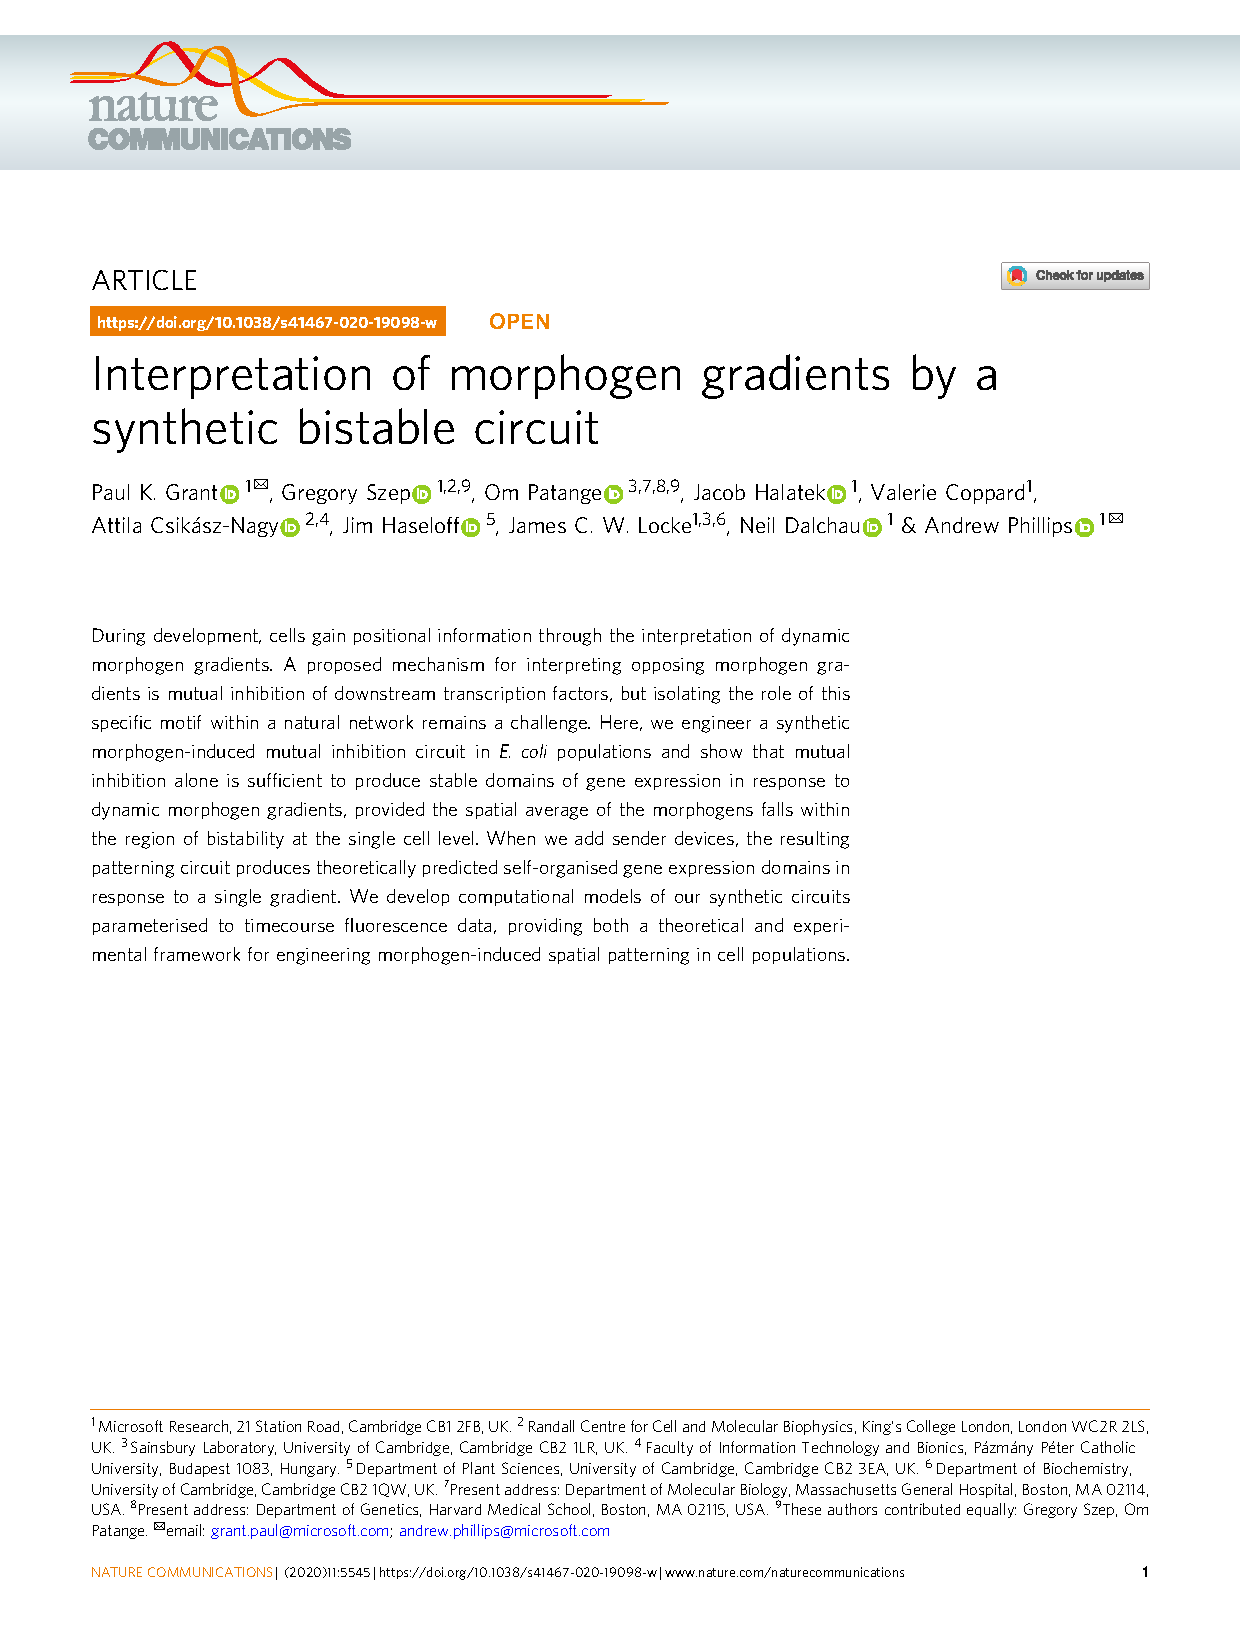
\includepdf[pages=1-8, offset=75 -90, scale=0.85, frame,
        clip,trim=10mm 5mm 10mm 0mm,
        pagecommand={}, addtotoc={
        1,section,1,Abstract,double-exclusive:abstract,
        2,section,1,Introduction,double-exclusive:introduction,
        2,section,1,Results,double-exclusive:results,
        2,subsection,2,Engineering mutual exclusivity,double-exclusive:exclusivity,
        3,subsection,2,Mutual inhibition results in bistability,double-exclusive:bistability,
        4,subsection,2,Hysteresis produces stable boundaries,double-exclusive:boundaries,
        4,subsection,2,A secondary gradient creates self-organised domains,double-exclusive:self-organisation,
        5,section,1,Discussion,double-exclusive:discussion,
        6,section,1,Methods,double-exclusive:methods,
        6,subsection,2,Plasmid construction,double-exclusive:plasmids,
        6,subsection,2,Plate fluorometer assay,double-exclusive:plates,
        6,subsection,2,Flow-cytometric analysis of hysteresis,double-exclusive:flow,
        7,subsection,2,Microfluidics,double-exclusive:microfluidics,
        7,subsection,2,Microfluidics microscopy,double-exclusive:microscopy,
        7,subsection,2,Solid culture assays,double-exclusive:cultures},
    addtolist={
        2, figure, {\textit{Fig. 1}\quad A synthetic gene circuit for morphogen interpretation.}, fig:double-exclusive:overview,
        3, figure, {\textit{Fig. 2}\quad Mutual inhibition produces bistability.}, fig:double-exclusive:bistability,
        5, figure, {\textit{Fig. 3}\quad Formation of stable boundaries.}, fig:double-exclusive:boundaries,
        6, figure, {\textit{Fig. 4}\quad Addition of a Relay circuit creates self-organised domains of gene expression.}, fig:double-exclusive:relay
}]{publications/double-exclusive.pdf}

\section{Afterword}

The decision to focus on single cell trajectories and flow cytometry in this study came from the limitations of using microplate data: it is not possible to detect multi-modality in fluorescence distributions from plates that could indicate a population of mixed phenotypes. In order to restore phenotype information, model parameters $\theta$ were estimated using a hierarchical Monte Carlo approach and time-course fluorescence microplate measurements (details of which can be found in Appendix \ref{appendix:double-exclusive:inference}). Unfortunately time-courses include information about dynamical transients and colony growth in liquid culture. The desired cusp bifurcation, however, lives in state-space rather than the time-domain. It is not possible to observe the cusp bifurcation in microplate data due to the averaging of signals originating from heterogeneous cell populations. Instead, the cusp bifurcation can be observed in flow cytometry measurements of colonies in exponential phase (Supplementary Figure \ref{fig:double-exclusive:flow-hysteresis}) and microfluidic fluorescence microscopy data (Figure \ref{fig:double-exclusive:bistability}c) where computations on single-cell trajectories reveal the hysteresis loop which must necessarily accompany the cusp. The disconnect between the domain that the data lives in and the domain of the design goals poses the risk of over-fitting the model on undesired information that exists in the data domain.

This motivated investigating \emph{inverse bifurcation analysis} methods that could try and find parameter regimes that lead to desired cusp and limit points directly. However, searching for bifurcating parameter regimes within a model is a difficult task, and few methods exist in the literature. We found some contributions where bespoke methods were applied to specific model structures, but would not generalise to arbitrary models \cite{}. Other approaches were based on sampling parameter sets naively and checking for the existence of a bifurcation \cite{}. But, there was no end-to-end differentiable method that took advantage of bifurcation theory directly. We therefore attempted to fill this gap in the literature by developing a methodology based on differentiable continuation in Chapter \ref{chapter:inference}. In doing so, we have elucidated the importance of fitting qualitative before quantitative features within datasets.
\chapter{Parameter Inference with Bifurcation Diagrams}
\label{chapter:inference}
\epigraph{``No person will deny that the highest degree of attainable accuracy is an object to be desired, and it is generally found that the last advances towards precision require a greater devotion of time, labour, and expense, than those which precede them."}{Charles Babbage}

\section{Preface}
\begin{enumerate}
    \item How does this paper address limitations of Chapter \ref{chapter:double-exclusive} 
    \item Alternative approaches
\end{enumerate}

In this section a single iteration of the model reduction loop
outlined in Section \ref{section:refinement}
is bench-marked against synthetic data that represent noisy single cell
gene expression trajectory data. The results show how one could start
with a hypothesis containing 30 parameters, and end up with only
7 relevant parameters after one iteration.

\subsection{Synthetic Data Generation}
The Euler-Maruyama method is used to generate $N/K$ points per
trajectory for $K$ trajectories  from a ground truth field $\Vector{g}$ with a
specific signal to noise ratio $\alpha$. The dataset 
$\mathcal{D}=\{\Vector{u}_1^1\dots\Vector{u}_{N/K}^K\}$ is obtained by
\vspace{-1em}
\begin{align}
    \Vector{u}_{n+1}^k =
    \Vector{u}_{n}^k +\Vector{g}(\Vector{u}_{n}^k)\Delta t
    +\frac{1}{\alpha}|\Vector{g}(\Vector{u}_{n}^k )|\Delta W\\
    \text{for given initial conditions}\quad\Vector{u}_{1}^1 \dots \Vector{u}_{1}^K\nonumber\\
    \Delta W \sim \mathcal{N}(0,\sqrt{\Delta t})\qquad\qquad
\end{align}
where $\Delta t$ is a sufficiently small chosen timestep, and $\Delta W$ is a Wiener
process, distributed normally with a mean of zero and standard deviation of $\Delta t$.
Figure \ref{fig:sample-data} shows example data generated from uniform cycle field
\begin{equation}
    \Vector{g}(x,y)=\frac{1}{\sqrt{x^2+y^2}}
    \begin{pmatrix}
    -y \\ x
    \end{pmatrix}
    \label{eq:cycle-field}
\end{equation}
\vspace{-2em}
\begin{Figure}
\includegraphics[width=70mm]{figures/sample-data-2.png}
\includegraphics[width=70mm]{figures/sample-data-3.png}
\caption{\textcolor{Emerald}{Datasets} $\mathcal{D}$ generated from cycle field \eqref{eq:cycle-field}
for $K=7$ initial \\conditions. Signal to noise ratios are $\alpha=10,\sqrt{10}$
on left, right respectively}
\label{fig:sample-data}
\end{Figure}

\subsection{Non-parametric Inference with Gaussian Processes}
A non-parametric estimate of the vector field $\Vector{f}(\Vector{u})$ can be
obtained by assuming $\mathcal{D}$ is generated by a Gaussian process.
This requires the inversion of an $N\times N$ data matrix which has a computational
complexity $N^3$ which is only tractable with sparse datasets. Since top-down
feature specification is indeed sparse and it is always possible to partition
and down-sample larger datasets, this approach is appropriate for our given
objectives. Let the region $\partial\mathcal{D}$ be defined by the Delaunay tessellation of the
input data $\mathcal{D}$. The inferred field is defined only within the region
$\partial\mathcal{D}$ to minimise basis function artefacts.
\begin{equation}
    \Vector{f}(\Vector{u})\sim
        \mathcal{N}(\,\Vector{\mu}(\Vector{u}) ,\Matrix{\Sigma}(\Vector{u})\,)
    \quad\mathrm{for}\quad\Vector{u}\in\partial\mathcal{D}
\end{equation}\\
where at any given state $\Vector{u}$ the field is generated by Gaussian
distributions of mean vector $\Vector{\mu}(\Vector{u})$ and covariance matrix $\Matrix{\Sigma}(\Vector{u})$.
Solving for these requires a choice of matrix-valued kernel function $\Matrix{K}(\Vector{u},\Vector{v})$
which encodes our knowledge about the local structure of the field.
Sophisticated kernels for learning vector fields exist \cite{Fuselier2017ADecompositions} for decomposing
fields in conservative and solonoidal components, which aid in localising fixed points and
limit cycles. The simplest choice of kernel assumes the components are independent
and have a finite correlation length $\gamma$, such as Gaussian radial basis functions.
Here $\Matrix{I}$ is the identity matrix and the hyperparameter $\gamma$ has to be optimised.
\begin{equation}
    \Matrix{K}(\Vector{u},\Vector{v}) = \Matrix{I}\,\mathbb{e}^{-\gamma|\Vector{u}-\Vector{v}|^2}
\end{equation}
The geometric error $E$ between the inferred field $\Vector{f}$ and the ground truth $\Vector{g}$ at a specific
location in state space $\Vector{u}$ is a quatifty that should be zero
when the fields are pointing in the same direction and one when they are pointing in opposite
directions. Hence the use of the dot product
\begin{align}
    E(\Vector{f}|\Vector{g}) :=
    \frac{1}{2}
    \left(1-\frac{\Vector{f}\cdot\Vector{g}}{|\Vector{f}||\Vector{g}|}\right)\qquad\qquad\quad\\
    = \frac{1-\cos\theta}{2}\quad\text{where $\theta$ is the angle between $\Vector{f}$ and $\Vector{g}$}
\end{align}
Figure \ref{fig:inferred-cycles} shows inferred fields using the
$\pythoninline{GaussianProcessRegressor()}$ class from $\pythoninline{sklearn}$
\cite{Seeger2004GaussianLearning.} from data generated from \eqref{eq:cycle-field}.
Its clearly visible the field inference fails outside the data region $\partial\mathcal{D}$,
justifying the desire to only define the inferred result within the region. It can
also be seen that data generated with a lower signal-to-noise ratio $\alpha$ may
results larger geometric mismatches within the data region. Figure \ref{fig:inferred-at-snr}
reveals the robustness of this proceedure with respect to noise, showing a
consistent mean error below $16\%$. However this does not necessarily mean that
global dynamics are of the inferred field match that of the ground truth. In the
right sub-figure of Figure \ref{fig:inferred-cycles} it can be seen that the noisy
trajectories induce a stable fixed point at their centre.

\begin{Figure}
\includegraphics[width=70mm]{figures/cycle-2.png}
\includegraphics[width=70mm]{figures/cycle-1.png}
\caption{Gaussian process regressors inferring fields from \textcolor{Emerald}{cycle data} $\mathcal{D}$ with varying signal to noise ratios. Error $E$ is shown as a heatmap on \textcolor{orange}{inferred fields}  $\Vector{f}$ 
within the data region $\partial\mathcal{D}$.}
\label{fig:inferred-cycles}
\end{Figure}
\vspace{-2em}
\begin{Figure}
\includegraphics[width=80mm]{figures/cycle-snr.png}
\caption{Mean geometric error of the inferred field $\Vector{f}$ as a function\\
of signal-to-noise ratio $\alpha$ used to generate data $\mathcal{D}$}
\label{fig:inferred-at-snr}
\end{Figure}

\subsection{Geometric Inference of Parameters}
Suppose an accurate non-parametric representation $\Vector{f}$ of the observations
$\mathcal{D}$ or top-down specified hypothesis $\mathcal{H}$ has been obtained.
This section outlines a method by which parametric hypotheses
$\Vector{h}(\Vector{\theta})$ can be matched to $\Vector{f}$, and to what extent
parameters $\Vector{\theta}$ are relevant in matching the it. In order to
to this the following geometric cost function $\mathcal{L}(\Vector{\theta})$ must
be minimised
\begin{align}
    \mathcal{L}(\Vector{\theta}) &:= \mathbb{e}^{E(\Vector{f}|\Vector{h}(\Vector{\theta}))}
    +\lambda ||\Vector{\theta}||\\
    &= \sqrt{\mathbb{e}}\,
    \mathbb{e}^{-\frac{\Vector{f}\cdot\Vector{h}(\Vector{\theta})}
    {|\Vector{f}||\Vector{h}(\Vector{\theta})|}}
    +\lambda ||\Vector{\theta}||
\end{align}
where $\lambda$ is a regularisation hyperparameter and $||\Vector{\theta}||$ is some
norm with respect to the parameters. This norm encodes our prior assumptions on
what parameters we expect to find or wish to find. To reduce the complexity of
the inferred hypothesis, it should be assumed that as many parameters as possible
are zero. This can be done by choosing the $\ell_1$ norm for regularisation. Suppose
the hypothesis takes a mass-action form, then one could express the field as
\begin{equation}
    \Vector{h}(\Vector{\theta})=\Matrix{\Theta}\,\Vector{\phi}
    \quad\text{where}\quad\Vector{\phi}:=(u_1, u_2, u_1 u_2, u_1^2\,...\, )
\end{equation}
where the the parameter matrix $\Matrix{\Theta}$ multiplies a polynomial feature
vector $\Vector{\phi}$. Figure \ref{fig:convergence} shows a convergening optimisations
of $\mathcal{L}(\Vector{\theta})$ for the above hypothesis $\Vector{h}(\Vector{\theta})$
against the ground truth field given by \eqref{eq:cycle-field} using $\pythoninline{scipy.optimize.minimize(method='SLSQP')}$. It is possible to identify sloppy
vs stiff parameters by ordering them according to their variance from model to model.
Most parameters are stiff and zero as set by the regularisation, leaving non-zero
parameters which are either stiff or sloppy. Upon closer inspection of the sloppy
parameters $\Vector{s}\in\Vector{\theta}$ it can be deduced that 
\begin{equation}
    \Vector{z}=\Matrix{W}\,\Vector{s}
\end{equation}
where $\Matrix{W}$ is a sparse rectangular matrix that constructs linear combinations
of sloppy parameters to minimise the variance of the output $\Vector{z}$. There are
several decomposition algorithms that one could use to obtain this matrix $\Matrix{W}$
such as Independent Component Analysis. Figure \ref{fig:indepedent} reveals that
the terms indeed are only sloppy to preserve their sums or differences. Out of 30
parameters inferred this procedure suggests that only 7 of them are relevant for
model construction.

\begin{Figure}
\includegraphics[width=70mm]{figures/convergence.png}
\includegraphics[width=70mm]{figures/parameters.png}
\caption{Left: convergence loss minimisation $\mathcal{L}(\Vector{\theta})$ for 100 initialisations of
of the parameter vector $\Vector{\theta}$ Right: Final parameters for each obtained model,
revealing sloppy and stiff terms}
\label{fig:convergence}
\end{Figure}

\begin{Figure}
\includegraphics[width=70mm]{figures/indepedent.png}
\caption{Independent component analysis applied to the sloppy terms $\Vector{s}$.\\
The independent terms are either sums or differences of the sloppy terms.}
\label{fig:indepedent}
\end{Figure}
\newpage
\subsection{Basis Function Models}
Parametric models such as mass-action are can be expressed as
\begin{equation}
    \partial_t\Vector{u}(t) = \Matrix{\Theta}\,\Vector{\phi}(\Vector{u})
\end{equation}
the nullclines are
\begin{equation}
    \Matrix{\Theta}\,\Vector{\phi}(\Vector{u}) = 0
\end{equation}
suggesting isotropically re-scaling the parameters
doesn't change the location of the nullclines $\Matrix{\Theta}\rightarrow\alpha\Matrix{\Theta}$
where $\alpha$ is positive definite.

\includepdf[pages=1-11, offset=75 -95, scale=0.85, frame,
        clip,trim=31mm 21mm 31mm 21mm,
        pagecommand={}, addtotoc={
        1,section,1,Abstract,inference:abstract,
        1,section,1,Introduction,inference:introduction,
        2,subsection,2,Preliminaries,inference:preliminaries,
        4,section,1,Proposed Method,inference:method,
        4,subsection,2,Semi-supervised Cost Function,inference:cost,
        5,subsection,2,Differentiating the semi-supervised cost function,inference:derivatives,
        6,section,1,Experiments \& Results,inference:results,
        6,subsection,2,Minimal Models,inference:minimal,
        6,subsection,2,Genetic Toggle Switch,inference:genetic,
        7,subsection,2,Complexity,inference:complexity,
        9,section,1,Conclusion \& Broader Impact,inference:impact,
        9,section,1,Acknowledgements,inference:acknowledgements},
    addtolist={
        3, figure, {\textit{Fig. 1}\quad Illustration of bifurcation diagrams for minimal models of bifurcations. A. Saddle-node bifurcations arise for $\rates(u,p) = p + \theta_{1}u+\theta_{2}u^3$ when $\theta = (\frac{5}{2},-1)$. B. Pitchfork bifurcations arise for $\rates(u,p) = \theta_{1} + p u+\theta_{2}u^3$ when $\theta=(\frac{1}{2},-1)$. Targets are illustrated by light yellow vertical lines. Bifurcation curves are shown as solid blue and red lines, with lighter shades indicating the determinant crossing zero at locations $\predictions(\theta)$ giving rise to unstable solutions.}, figure:inference:minimal-models,
        4, figure, {\textit{Fig. 2}\quad Bifurcation measure $\measure(s)$ and determinant $\Det$ along the arclength $s$ of two different bifurcation curves demonstrating how maximising the measure along the curve maintains the existing bifurcation marked by a circle, while encouraging new bifurcations marked by stars.}, figure:inference:measure,
        7, figure, {\textit{Fig. 3}\quad Saddle-node $\rates(u,p) = p + \theta_{1}u+\theta_{2}u^3$ and pitchfork $\rates(u,p) = \theta_{1} + u p +\theta_{2}u^3$ optimised with respect to $\theta$ so that predicted bifurcations $\predictions(\theta)$ match targets $\targets$ in control condition $p$. The right panel shows bifurcations diagrams for the three optimal $\theta^*$ marked by stars on the left panel. The optimisation trajectories in white follow the gradient of the cost, approaching the black lines of global minima in the left panel}, figure:inference:minimal-models:results,
        8, figure, {\textit{Fig. 4}\quad Bifurcation inference for the two-state model (11). A. Optimal parameter estimates $\theta^*$ for the targets $\targets=\{4,5\}$ reveal two clusters of qualitatively different regimes: mutual activation ($a_1 < 1$; cluster 1) and mutual inhibition ($a_1 > 1$; cluster 2). B. Example bifurcation diagrams indicate positively and negatively correlated dependencies between the two model states, as a function of the control condition.}, figure:inference:two-state-optima,
        8, figure, {\textit{Fig. 5}\quad Complexity scaling of calculating the gradient of the cost function. Calculations were performed on an Intel Core i7-6700HQ CPU @ 2.60GHz x 8 without GPU acceleration}, figure:scaling
}]{publications/bifurcation-inference.pdf}
\chapter{Exploring bifurcations between phenotypes}
\label{chapter:exploring}

\chapter{Conclusions}
\label{chapter:conclusions}
\begin{music}
    \parindent10mm \instrumentnumber{1} \setstaffs1{1} 
    \generalmeter{\meterfrac34} \generalsignature{-1}
    \startextract
		\notes  \en
    \zendextract
\end{music}
\epigraph{\textit{A childish mind will turn to noble ambition}}{Ocarina of Time}

\section{Retrospectives}

In this thesis we explored the relationship between an organism phenotype and bifurcations in differential equations models seeking to model the organism behaviour. In the collaboration in synthetic biology in chapter \ref{chapter:double-exclusive}, the experimental design goals were to engineer a particular phenotypic behaviour of \emph{E. coli}. This amounted to designing particular bifurcations in the corresponding differential equation model. A gap in machine learning methods for differential equations that optimise with respect to targets directly in state space was identified, leading to the proposed method in Chapter \ref{chapter:inference}. We laid the foundations for methods that learn differential equation models that match qualitative behaviours and high-level constraints in state space. With this new method now in hand, we revisit how the collaboration in synthetic biology would have benefited and propose a \emph{Design-Learn} workflow that we argue would benefit any collaboration which designs phenotypes by iterative genetic manipulation of an organism \cite{Dalchau2018}. Differential equation models for an organism behaviour are not always available, as in the collaboration in immunology in chapter \ref{chapter:exploring}. We outlined the importance of interactive exploration and refinement of annotations of high-dimensional data clouds and built \emph{FlowAtlas.jl} to enable immunophenotyping across datasets with heterogeneous experimental designs. Our retrospectives are concluded with a vision of how methods from chapter \ref{chapter:exploring} can be used together with our proposed \emph{Design-Learn} workflow to organise and reduce different models of organisms whose behaviours can be experimentally captured with flow cytometry.

\subsection{A \emph{Design-Learn} workflow for synthetic biology}

One of the main insights from our collaboration in synthetic biology is the importance of the representation of the observed data in tuning the learned aspects of a hypothesis. The data representation must be invariant under  transformations that we do not want to learn. When engineering \emph{E. coli} we did not care about timescales or dynamical transients in the organisms response to experimental inputs. We also did not care about the exact concentrations of fluorescent proteins at steady state. The main concern was designing the shape of the bistable region in the experimental inputs.

This motivates processing flow cytometry data using basis function methods (Section \ref{section:basis-function-methods}) and running co-dimension two continuation methods to extract the limit curve that defines the separatrix between monostable and bistable regions in state space. The limit curve tells us where the steady state manifold folds, and can then be used as target data $\targets$ to infer parameters $\theta$ of some hypothesis $\rates$ using the method in Chapter \ref{chapter:inference}. Alternatively, one optimise $\theta$ with respect to a geometric cost \eqref{eq:geometric-cost} that compares the field estimated from data $F$ to some parametrised hypothesis $\rates$. While kinetic information is ignored in this method, modes in the fluorescence distributions in the flow cytometry data define the locations of fixed points, and hence the shape of the steady state manifold. Whether design goals involve the whole shape of the steady state manifold or just its fold locations, a non-parametric representation $F$ of the data is required. Once the optimal parameters $\theta^*$ are obtained, the experimentalist can explore the neighbourhood of $\theta^*$ and see how they can change the bistable region, or whether they are close to another bifurcation which would produce a new phenotype. This can lead to new experiments that change the genotype $\theta^*+\Delta\theta$ in attempts to produce new phenotypes. Changes in genotype can involve promoter engineering for modulating transcription rates \cite{}, using degradation tags to change degradation rates \cite{} or ribosome binding site engineering for controlling translation \cite{}. The new data in turn can be used to refine the hypothesis; a summary of such a \emph{Design-Learn} pipeline is presented in Figure \ref{fig:deisgn-learn}.
\begin{Figure}
	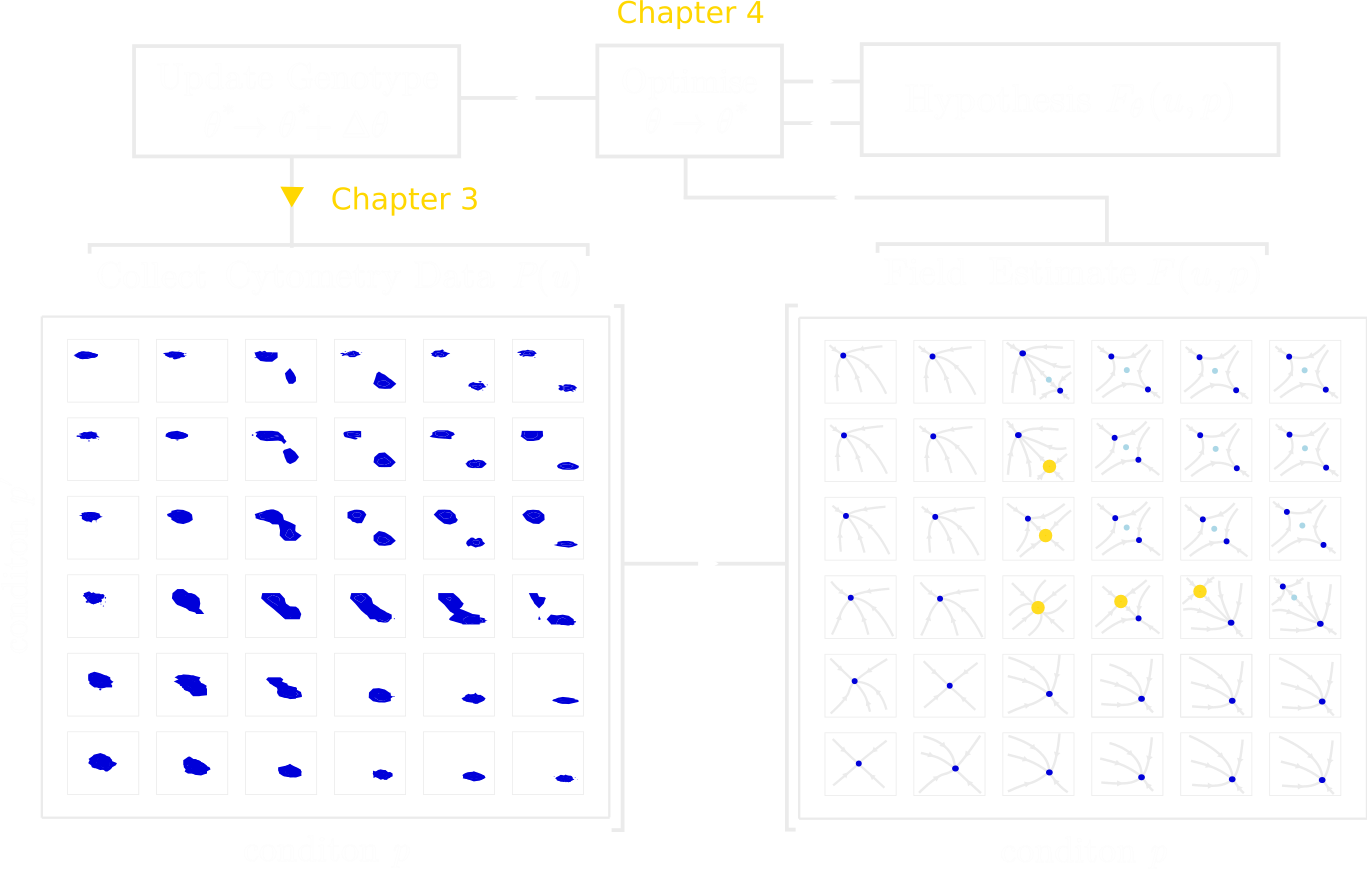
\includegraphics[width=\linewidth]{design-learn}
	\caption{Overview for a \emph{design-learn} workflow, developed in hindsight, for genetic design of the \emph{double exclusive reporter}. Non-parametric estimates of the field $F(u,p)$ yield state space geometry from cytometry data. A parametrised hypothesis $\rates(u,p)$ is then optimised against the data-driven state space geometry, to obtain optimal parameters $\theta^*$. The neighbourhood of $\theta^*$ is then investigated to decide which genetic modifications lead to improved designs, which are then tested with subsequent collection of more cytometry data.}
	\label{fig:deisgn-learn}
\end{Figure}
Approaches that do not require a non-parametric field $F$ to obtain target bifurcations $\targets$ involve quantifying the variance around clusters in the flow cytometry data. In the vicinity of bifurcations we expect certain scaling laws to emerge (Section \ref{section:fluctuations}) and localising bifurcations would require identifying such laws. A simple approach to this would be to localise cluster splitting, which was explored in Chapter \ref{chapter:double-exclusive} but never used to produce targets $\targets$ for optimisation. Accurate localisation of bifurcations using these methods require fine experimental sampling along the control condition $p$ and can ultimately be limited by intrinsic noise in the organism.

\subsection{Bifurcations \& model reduction}

\emph{E. col} is a relatively simple organism whose genetic components can be individually modelled with biochemically reasonable assumptions and catalogued in a library of parts. This is not the case for the human immune system which was explored in chapter \ref{chapter:exploring}.

\section{Future Work}

We now discuss future directions that would use this thesis as a starting point, in particular 

\subsection{Designing Limit Cycles}

\subsection{Spatially Extended Systems}

\section{Limitations \& Alternative Approaches}

\addcontentsline{toc}{chapter}{Appendices}
\appendix

\chapter{Interpretation of Morphogen Gradients by a Bistable Circuit}
\label{appendix:double-exclusive}
\includepdf[pages=1-51, offset=75 -90, scale=0.85, frame,
        clip,trim=20mm 5mm 20mm 15mm,
        pagecommand={}, addtotoc={
                2,section,1,Supplementary Figures,appendix:double-exclusive:figures,
                18,section,1,Supplementary Methods,appendix:double-exclusive:methods,
                19,subsection,2,Differential Equation Models \& Parameter Inference,appendix:double-exclusive:inference,
                40,subsection,2,Bistability Analysis,appendix:double-exclusive:bistability,
                42,subsection,2,Boundary Experiments,appendix:double-exclusive:boundaries,
                50,subsection,2,Models of the Exclusive Receiver Relay Circuits,appendix:double-exclusive:relay},
        addtolist={
                2, figure, {\textit{Supplementary Figure 1}\quad Circuit variants}, fig:double-exclusive:variants,
                4, figure, {\textit{Supplementary Figure 2}\quad Raw timecourse fluorescence traces}, fig:double-exclusive:plate-data,
                15, figure, {\textit{Supplementary Figure 13}\quad Hysteresis flow cytometry experiments}, fig:double-exclusive:flow-hysteresis,
                41, figure, {\textit{Supplementary Figure 25}\quad Bifurcation curves for uniform and protected degradation models}, fig:double-exclusive:degradation-models,
                41, figure, {\textit{Supplementary Figure 26}\quad ifurcation curve insensitivity specific growth rate $\gamma_0$}, fig:double-exclusive:growth-rate-sensitivity
}]{publications/double-exclusive-si.pdf}

\chapter{Parameter Inference with Bifurcation Diagrams}
\label{appendix:inference}
\includepdf[pages=1-6, offset=75 -90, scale=0.85, frame,
        clip,trim=33mm 20mm 33mm 20mm,
        pagecommand={}, addtotoc={
                1,section,1,Bifurcation Diagrams as Tangent Fields,appendix:tangent-fields,
                2,section,1,Bifurcation Measure Properties,appendix:bifurcation-measure,
                3,section,1,Leibniz Rule for Space Curves,appendix:leibniz-rule,
                5,section,1,Application to the Double Exclusive Model,appendix:more-complex-model,
                6,section,1,Extension for Hopf Bifurcations,appendix:hopf-measure},
        addtolist={
                1, figure, {\textit{Supplementary Figure 1}\quad Two implicit surfaces $f_{\theta}(z)=0$ and $g_{\theta}(z)=0$ in $\mathbb{R}^3$ intersecting to form a space curve which is tangent to field $\tangent(z)$ and perpendicular to gradients $\partial_{z}f_{\theta}$ and $\partial_{z}g_{\theta}$}, fig:implicit-surfaces,
                2, figure, {\textit{Supplementary Figure 2}\quad Left/Right : Determinant $\Det$ and tangent field $\tangent(z)$ for the saddle-node/pitchfork models for some set values of $\theta$ revealing that $\Det=0$ defines bifurcations}, fig:determinant-field,
                5, figure, {\textit{Supplementary Figure 3}\quad Bifurcation inference for the \emph{double exclusive reporter}. A. Optimal parameter estimates $\theta^*$ for the targets $\targets=\{1,2\}$ (indicated by yellow lines in panel B) reveal four regions  with two geometrically different regimes: mutual activation (region 1) and mutual inhibition (regions 2-4). B. Example bifurcation diagrams indicate that region 2 has swapped kinetics between $L$ and $T$ to region 3. Region 4 has models with non-zero imaginary parts to eigenvalues indicating damped oscillations (shown in light green).},
                fig:double-exclusive-optima,
                6, figure, {\textit{Supplementary Figure 4}\quad Bifurcation measure $\measure(s)$ and eigenvalues $\lambda(s)$ along the arclength $s$ for two different bifurcation curves demonstrating how the measure detects non-zero imaginary parts $\Imag[\lambda]$ (onset of damped oscillations marked by circle) and sign changes in real parts $\Real[\lambda]$ (Hopf bifurcations marked by stars)},
                fig:hopf-measure
}]{publications/bifurcation-inference-si.pdf}

\chapter{Exploring Bifurcations between Phenotypes}
\label{appendix:exploring}

\section{Experimental Methods}
\subsection{Tissue Acquisition \& Dissociation} 

All samples were collected via the \href{https://www.cbtm.group.cam.ac.uk}{Cambridge Biorepository for Translational Medicine} under Research Ethics Committee approval 15/EE/0152. Tissue was obtained from five deceased organ donors following circulatory death. Donor metadata is given in Table \ref{table:donors}. Briefly, following cessation of circulatory function donors proceeded to organ donation. Organs were perfused \emph{in situ} with cold organ preservation solution and cooled with topical application of ice. Samples for the study were obtained within 60 minutes of cessation of circulation and placed in University of Wisconsin organ preservation solution for transport at 4°C to the laboratory. Lung and liver samples were obtained from the left lower lobe of the lung and the right lobe of the liver. In addition, two donor-matched blood samples were collected prior to withdrawal of life support, under approval 97/290.

To minimise the possibility of processing-depended differences in cell surface marker expression, all samples, including blood, were processed using enzymatic digestion protocol. Briefly, solid tissues were weighed, transferred into 10cm tissue culture dishes and cut into small pieces. Up to 5g of tissue was then transferred to each of eight GentleMACS C tubes (Miltenyi Biotec) containing 5mL of dissociation media composed of X-vivo15 supplemented with 0.13U/mL Liberase TL (Roche), 10U/mL Benzonase nuclease (Millipore/Merck), 2\% (v/v) heat-inactivated fetal bovine serum (FBS, Gibco), penicillin (100 U/ml, Sigma-Aldrich), streptomycin (0.1 mg/ml, Sigma-Aldrich), and 10mM HEPES (Sigma Aldrich). The samples were then dissociated on a GentleMACS Octo dissociator (Miltenyi Biotec) running a protocol that provided gradual ramping up of homogenisation speed and two 15 minute heating/mixing steps at 37°C. Digested tissue was passed through a 70$\mu$m MACS Smartstrainer (Miltenyi Biotec) and the flow-through was first washed with media supplemented with 2 mM EDTA and then with PBS. Mononuclear cells were enriched by Ficoll-Paque (GE Healthcare) density centrifugation according to manufacturer's instructions. Following, density centrifugation, mononuclear layer was collected, washed once with PBS and cell pellet was resuspended in FACS buffer (PBS, 2.5$\%$ FBS).

Bone marrow aspirates and peripheral blood samples were first subjected to Ficoll-Paque density centrifugation, according to manufacturer's instructions, the mononuclear layer was then collected, washed with PBS and cells were treated with the same dissociation media as solid tissues for 30 min at 37°C prior to washing and resuspension in FACS buffer.

\subsection{Flow Cytometry}

Depending on the cell yield, up to 1x10\textsuperscript{6} mononuclear cells/tissue were stained with antibodies shown in Table \ref{table:panel}. Not all donors were stained with the same panel. To expand total number of markers, sentinel panel design was implemented where CD3 and IgD were detected with antibodies conjugated to BUV395 and Foxp3 and IgM were detected with antibodies conjugated to PE in some donors. Refer to Table \ref{table:panels} for details. 

Single cell suspensions were washed once in PBS, transferred into 96 v-bottom plate and stained with Zombie UV viability dye for 30 min at 4°C following by a wash with FACS buffer. Cell pellets were resuspended in 50$\mu$l FACS buffer with Human FcR block (BD Biosciences) and incubated for 10 min at 4°C. Next, cells were pelleted, excess buffer removed and 100$\mu$l of antibody master mix composed of cell-surface antibody cocktail (see Table \ref{table:panels}), BV buffer (BD) and True-Stain Monocyte Blocker (Biolegend) and incubated for 1h at 4°C. Following incubation, cells were washed three times in PBS and prepared for intracellular staining using transcription factor fixation/permeabilisation kit (eBioscience) according to the manufacturer's instructions. Following IC staining, cell were resuspended in PBS and analysed on BD FACSymphony A3 cell analyser within 10 hours.

\section{Supplementary Tables}

\begin{landscape}
\begin{table}
\footnotesize
\begin{center}
\begin{tabular}{>{\centering\arraybackslash}p{0.6cm}>{\centering\arraybackslash}p{0.4cm}>{\centering\arraybackslash}p{0.7cm}>{\centering\arraybackslash}p{0.9cm}>{\centering\arraybackslash}p{0.9cm}>{\centering\arraybackslash}p{0.9cm}>{\centering\arraybackslash}p{1cm}>{\centering\arraybackslash}p{1cm}>{\centering\arraybackslash}p{1cm}>{\centering\arraybackslash}p{1cm}>{\centering\arraybackslash}p{2.1cm}>{\centering\arraybackslash}p{0.6cm}}
    \toprule
    Donor ID & Sex & Age & Primary cause of death & Multi-trauma & Days in hospital & BMI &CMV/ EBV/ TOXO& Smoking & Alcohol (u/day) & Antibiotics within 2 weeks of death & Steroids \\
    \midrule
    390C & F & 65-70 & ICH & \cmark & 2 & 30-35 & $+$/$+$/$-$ & ? & $<$1 & \xmark & \xmark \\
    403C & M & 50-55 & ICH & \cmark & 8 & 30-35 & $+$/$+$/$-$ & \cmark & $<$1 & Co, T & \xmark \\
    423C & M & 60-65 & ICH & \xmark & 2 & 20-25 & $-$/$+$/$-$ & \cmark & $>$9 & G, F & D \\
    412C & M & 70-75 & ICH & \xmark & 5 & 26-30 & $-$/$+$/$+$ & \cmark & $<$2 & A$^\star$ , F, G, C, Co & P$^\dagger$ \\
    428C & F  & 55-60 & ICH & \xmark & 3 & 20-25 & $-$/$+$/$-$ & \cmark & $>$9 & Co & \xmark \\
    \bottomrule
\multicolumn{12}{p{\linewidth}}{\vline height10pt width0pt
\relax F = Female; M = Male; ICH = intracranial haemorrhage; CMV = Cytomegalovirus; EBV = Epstein-Barr virus; TOXO = Toxoplasmosis; Co = Co-amoxiclav; A = Amoxicillin; T = Tazocin; F = Flucloxacillin; G = Gentamicin; D = Dexamethasone; C = Clarithromycin; \cmark = Yes; \xmark = No; ? = Not known;P = Prednisolone; $^\star$pre-admission, $^\dagger$pre-treatment}\\
\end{tabular}
\caption{Donor Metadata}
\label{table:donors}
\end{center}
\end{table}
\end{landscape}

\begin{table}
\footnotesize
\begin{center}
    \begin{tabular}{llll}
        \toprule
        Specificity & Fluorochrome & Clone & Source \\
        \midrule
        CD3 &  BUV395 & SK7 & BD \\
        CD8 & BUV563 & RPA-T8 & BD \\
        CD69 & BUV737 & FN50 & BD \\
        CD4 & BUV805 & SK3 & BD \\
        CD4 & BUV661 & SK3 & BD \\
        CD45 & BUV805 & HI30 & BD \\
        CD103 & BV421 & Ber-ACT8 & BD \\
        HLA-DR & BV510 & G46-6 & BD \\
        CD127 & PE-Cy7 & HIL-7R-M21 & BD \\
        CCR4 & BV605 & L291H4 & Biolegend \\
        CCR6 & BV650 & 11A9 & BD \\
        PD-1 & BV711 & EH12.1 & BD \\
        CD45RA & BV786 & HI100 & BD \\
        CCR10 & BB515 & 1B5 & BD \\
        CXCR3 & BB700 & 1C6/CXCR3 & BD \\
        CXCR5 & APC-R700 & RF8B2 & BD \\
        CCR7 & APC-Fire750 & G043H7 & Biolegend \\
        CD25 & APC & M-A251 & BD \\
        CD25 & APC & 2A3 & BD \\
        CD19 & BV570 & HIB19 & Biolegend \\
        IgM & PE & G20-127 & BD \\
        IgD & BUV395 & IA6-2 & BD \\
        Foxp3 & PE & 269D/C7 & BD \\
        Foxp3 & PE & PCH101 & eBioscience \\
        Helios & PE-Dazzle & 22F6 & Biolegend \\
        Zombie UV & - & - & Biologend \\
        \bottomrule
    \end{tabular}
\caption{Details of antibodies used in this study}
\label{table:panel}
\end{center}
\end{table}

\begin{table}
\footnotesize
\begin{center}
    \begin{tabular}{lrlll}
        \toprule
        & \multicolumn{4}{c}{Fluorochromes} \\
        \cmidrule{3-5}
         & Panels:&  A &  B &  C \\
        \cmidrule{3-5}
        Specificity & Donor:& 390C & 403C & 412C, 423C, 428C \\
        \midrule
        CD45 && BUV805 & - & - \\
        CD19 && - & - & BV570 \\
        IgM && - & - & PE \\
        IgD && - & - & BUV395 \\
        CD4 && \textbf{BUV661} & \textbf{BV805} & \textbf{BV805} \\
        CD3 &&  BUV395 & BUV395 & BUV395 \\
        CD8 && BUV563 & BUV563 & BUV563 \\
        CD69 && BUV737 & BUV737 & BUV737 \\
        CD103 && BV421 & BV421 & BV421 \\
        HLA-DR && BV510 & BV510 & BV510 \\
        CD127 && PE-Cy7 & PE-Cy7 & PE-Cy7 \\
        CCR4 && BV605 & BV605 & BV605 \\
        CCR6 && BV650 & BV650 & BV650 \\
        PD-1 && BV711 & BV711 & BV711 \\
        CD45RA && BV786 & BV786 & BV786 \\
        CCR10 && BB515 & BB515 & BB515 \\
        CXCR3 && BB700 & BB700 & BB700 \\
        CXCR5 && APC-R700 & APC-R700 & APC-R700 \\
        CCR7 && APC-Fire750 & APC-Fire750 & APC-Fire750 \\
        CD25 && APC & APC & APC \\
        Foxp3 && PE & PE & PE \\
        Helios && PE-Dazzle & PE-Dazzle & PE-Dazzle \\
        Zombie UV && Zombie UV & Zombie UV & Zombie UV \\
        \bottomrule
    \end{tabular}
\caption{Immunophenotyping panel designs used in the dataset}
\label{table:panels}
\end{center}
\end{table}

\bibliography{biblio}
\addcontentsline{toc}{chapter}{Bibliography}
\end{document}